\chapter{Approfondimento C}
\section{Funzioni di Libreria}
\subsection{Assert}
Cominciamo dicendo che \texttt{assert} non è una funzione di libreria,
anche se viene utilizzata nello stesso modo, ma è una \textbf{macro}. 
Essa prende in ingresso un'espressione e, se questa risulta falsa,
interrompe l'esecuzione del programma. Per utilizzarla:
\begin{verbatim}
#include <assert.h>
assert(exp); // espressione da valutare
\end{verbatim}
L'\texttt{assert} serve tipicamente per il \textbf{debug} e per verificare condizioni
interne del programma. In caso di errore, il programma viene terminato
(chiamando \texttt{abort()}).Se è definito \texttt{NDEBUG}, gli \texttt{assert} 
vengono disabilitati e non hanno effetto.
\subsection{Funzioni per la gestione di Stringhe}
Dato che C non offre delle funzioni per la gestione delle stringhe
è molto utile utilizzare delle funzioni esterne in base alle nostre esigenze,
come:
\begin{verbatim}
#include <string.h>
size_t strlen(const char* s);                          // calcola la lunghezza della stringa
char* strcpy(char *dst, const char* src);              // copia la stringa in un altra stringa
char* strncpy(char *dst, const char* src, size_t len); // copia la stringa fino al len 
                                                          carattere da src in dst. Se src
                                                          è più piccolo di dst i verranno riempiti
                                                          con il carattere '/0'. Mentre in caso 
                                                          di dst è più piccolo di src i 
                                                          caretteri andranno persi.
char* strcat(char* dst, const char* src);              // concatena le due stringhe
\end{verbatim}
\textbf{\textcolor{red}{ATTENZIONE:}} \texttt{dst} deve contenere abbastanza spazio
libero per contenere src
\begin{verbatim}
char* strtok(char* src, const char* delim); // divide la stringa in token
\end{verbatim}
Utilizzo:
\begin{verbatim}
    char* tocken= strtok(str, delim);
    while(token != null){
        .... codice che fa qualcosa con tocken
        tocken = strtok(NULL, delim);           // per andare al prossimo tocken
    }
\end{verbatim}
Vediamo però come funziona ogni parametro:
\begin{figure}[H]
    \centering  
    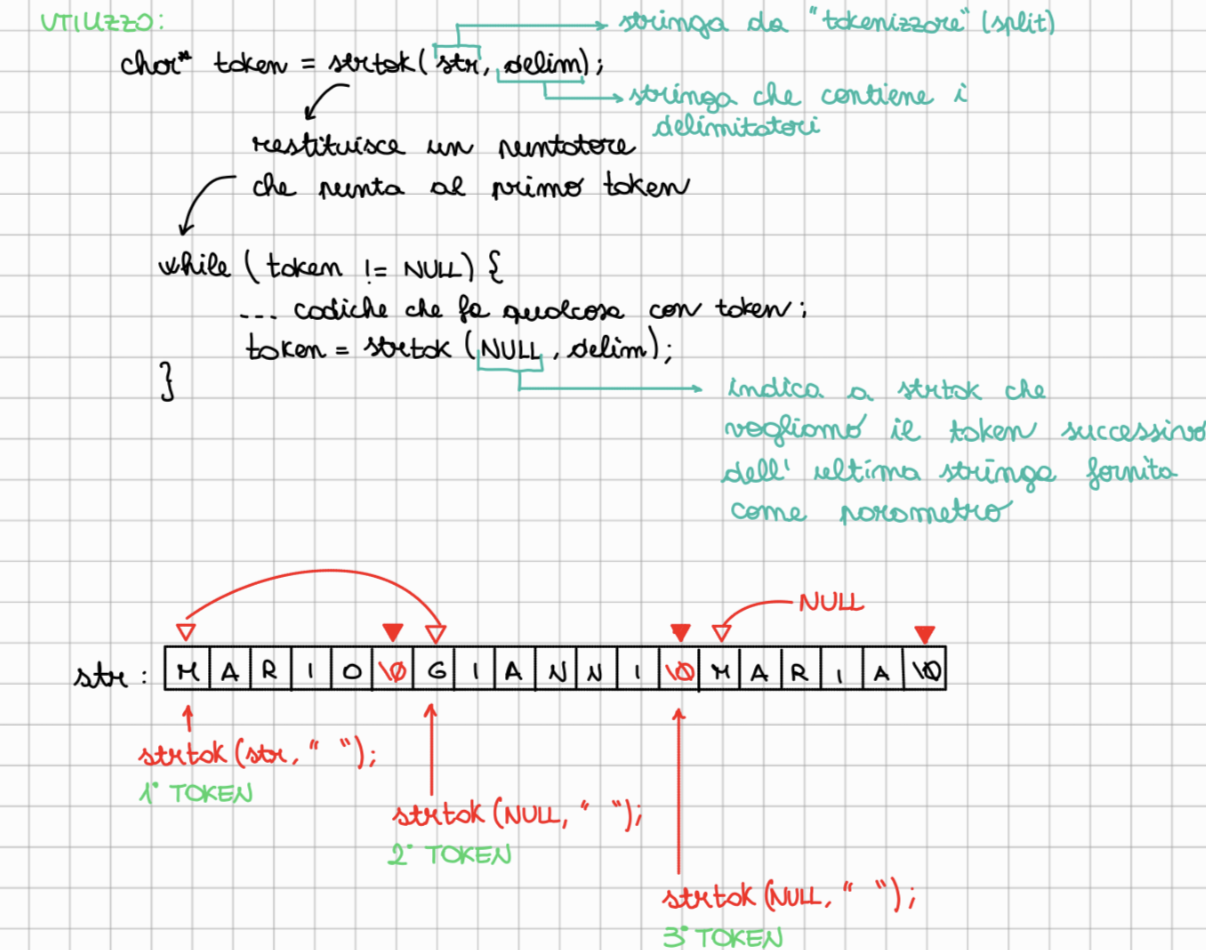
\includegraphics[width=0.9\linewidth]{../images/strtok.png}
    \caption{Funzionamento token}
    %\label{label}
\end{figure}
\noindent Vediamo ora un esempio di utilizzo:
\begin{verbatim}
    #DEFINE DELIM = ", "
    
    char* f(const char* s){
        char* temp = NULL;
        char* res = NULL;
    
        size_t len = strlen(s);
        char* tempo = malloc(sizeof(char)*(len+1));
        if(temp == NULL) goto cleanup;
        strncpy(temp, s, len);
        
        char* res = malloc(sizeof(char)*(len+1));
        if(res == NULL) goto cleanup;
        
        char* token = strtok(temp, DELIM);
        while(token){
            strncat(res, token, strlen(token));
            token = strtok(NULL, DELIM);
        }

        free(temp);
        retun res;
                
        cleanup:
        if(temp != NULL) free(temp);
        if(res != NULL) free(res);
        return NULL;
    }
\end{verbatim}
Utilizziamo il "\#DEFINE DELIM" per definire i delimitatori, in modo da 
non doverli riscrivere e poterci confondere.\medskip\\
Procediamo col vedere altre funzioni presenti nella libreria \texttt{string.h}:
\begin{verbatim}
int strcmp(const char* s1, const char* s2);
\end{verbatim}
Questa funzione confronta s1 ed s2 e restituisce: \medskip\\
$
\begin{cases}
    \textbf{$<$0} \text{        se s1 precede s2} \\
    \textbf{0}    \text{        se } s1 == s2 \\
    \textbf{$>$0} \text{        altrimenti}
\end{cases}
$\bigskip\\
Passiamo alla libreria \textbf{stdlib.h}:
\begin{verbatim}
#include <stdlib.h>
int atoi(const char* s); // converte s in un valore intero se possibile, altrimenti restituisce 0
\end{verbatim}
Esempio:
\begin{verbatim}
atoi("10");     --> 10
atoi("10abc");  --> 10
atoi("abc10");  --> 0 perchè non inizia con un numero
atoi("-10");    --> -10
\end{verbatim}
Esempio basilare di utilizzo:
\begin{verbatim}
void f(char* in[], int out[], int n){
    for(int i=0; i<n; i++)
        out[i] = atoi(in[i]);
}
\end{verbatim}
Vediamo ora degli esercizi dove otteniamo il minimo della lunghezza di due stringhe 
e un esercizio che verifica se un array di stringhe è ordinato o meno, utilizzando le funzioni viste
precedentemente:
\begin{verbatim}
int min_len(const char* a, const char* b){
    if(strlen(a)>=strlen(b))
        return strlen(a);
    else return strlen(b);
}

int is_sorted(char *v[], int n){
    for(int i=1; i<n; i++)
        if(strncmp(v[i-1], v[i], min_len(v[i-1], v[i])) > 0) return -1;
    return 0;
}
\end{verbatim}
Passiamo ora alal libreria \textbf{stdio.h}:
\begin{verbatim}
#include <stdio.h>
int sscanf(const char* s, const char* format, ...); 
\end{verbatim}
Questa funzione è simile a \texttt{scanf}, ma invece di leggere da standard input, legge da una stringa. 
Il primo parametro è la stringa da cui leggere, il secondo è il formato da utilizzare per la lettura, 
e i successivi sono i puntatori alle variabili dove salvare i valori letti.\\
Abbiamo poi la funzione \texttt{sprintf} che è simile a \texttt{printf}, ma invece di scrivere su standard output, scrive su una stringa.
Che fa sempre parte della libreria \textbf{stdio.h}:
\begin{verbatim}
int sprintf(char *d, const char* format, ...);
\end{verbatim}
Questa funzione scrive in d la stringa format formattata con i valori passati come argomenti, quindi:
il primo parametro è la stringa dove scrivere, il secondo è il formato da utilizzare per la scrittura, 
e i successivi sono i valori da scrivere.\\
Vediamo un esempio di utilizzo:
\begin{verbatim}
// converte una data da formato (input) "gg/mm/aaaa" a "mm/gg/aaaa"
int convert_date(const char *input, const char *output){
    int a,b,c;
    int res = sscanf(input, "%d/%d/%d", &a, &b, &c);
    if (res < 3) return -1;
    sprintf(output, "%d/%d/%d", b, a, c);
}
\end{verbatim}
Vediamo ora \texttt{getchar()}:
\begin{verbatim}
int getchar();                      // legge un carattere da standard input (da tastiera) 
                                        e lo restituisce come intero
int scanf(const char* format, ...); // legge da tastiera e salva i valori letti nelle 
                                        variabili passate come argomenti
\end{verbatim}
\subsection{Gestione della Memoria}
Vediamo ora come gestire la \textbf{memoria} in C.
\begin{itemize}
    \item \texttt{void *malloc(size\_t size)}; $\rightarrow$ alloca \texttt{size} byte di memoria e restituisce un puntatore a tale memoria. 
    Se l'allocazione fallisce, restituisce \texttt{NULL}.
    \item \texttt{void free(void *ptr)}; $\rightarrow$ libera la memoria precedentemente allocata con \texttt{malloc}.
    \item \texttt{void *calloc(size\_t count, size\_t size)}; $\rightarrow$ dove \texttt{count} indica il numero di 
    elementi da allocare e \texttt{size} la dimensione di ciascun elemento. Restituisce un puntatore alla memoria allocata, 
    inizializzata a zero.
    \item \texttt{void *memset(void *buf, int c, size\_t len)}; $\rightarrow$ imposta i primi \texttt{len} byte di \texttt{buf} 
    al valore del byte meno significativo di \texttt{c}. Restituisce un puntatore a \texttt{buf}.
    \item \texttt{void *memcpy(void *dst, const void *src, size\_t len)}; $\rightarrow$ copia \texttt{len} 
    byte da \texttt{src} a \texttt{dst}. Restituisce un puntatore a \texttt{dst}.\\ 
    \textbf{\textcolor{red}{ATTENZIONE:}} non usare su buffer che si sovrappongono.
        \begin{figure}[H]
        \centering  
        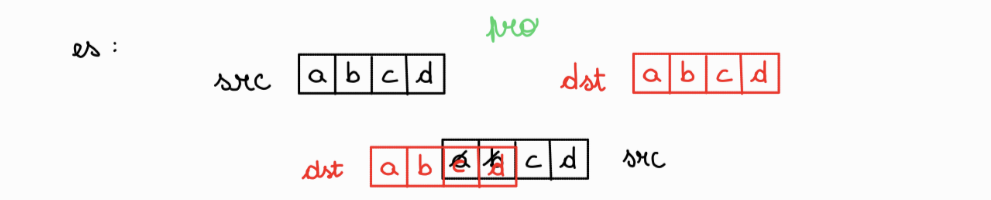
\includegraphics[width=0.9\linewidth]{../images/Buffer Sovrappongono.png}
        \caption{Esempio di buffer che si sovrappongono}
        %\label{label}
        \end{figure}
    \item \texttt{void *memmove(void *dst, const void *src, size\_t len)}; $\rightarrow$ copia \texttt{len} byte da \texttt{src} a \texttt{dst}. Restituisce un puntatore a \texttt{dst}.\\
    \textbf{\textcolor{red}{ATTENZIONE:}} può essere usato su buffer che si sovrappongono. Poichè src non viene mai sovrascritto.
\end{itemize}
Vediamo un esempio di utilizzo tramite una funzione bubblesort che ordina un 
array di stringhe di stessa lunghezza:
\begin{verbatim}
// buf buffer con all'interno stringhe, nel numero di stringhe presenti, size grandezza delle strighe
void bubblesort(void *buf, size_t nel, size_t size){
    char *tmp = buf;
    for(;;){
        for(int i = 1, i<nel; i++){
            int swap = 0; // variabile aggiuntiva per uscire dal ciclo
            strncmp(tmp+(i-1)*size,tmp+i*size, size) > 0{
                // scambio elementi
                swap_mem(tmp+(i-1)*size, tmp+i*size, size);
                swap = 1;
            }
        }
        // condizione di uscita poichè for infinito
        if(!swap) break;
    }
}
void swap_mem(void *s1, void *s2, size_t l){
    char *buf = malloc(l);
    if(buf == NULL) return;
    memmove(buf, s1, l); // copiamo s1 in buf
    memmove(s1, s2, l);  // copiamo s2 in s1
    memmove(s2, buf, l); // copiamo buf in s2
    free(buf);          // liberiamo la memoria allocata per buf
}
\end{verbatim}
Vediamo ora un ulteriore esempio di utilizo, tramite una funzione che indica il carettere
più frequente in un array buf di dimensione nel:
\begin{verbatim}
int most_freq_char(void *buf, size_t nel){
    int *c = malloc(sizeof(int)*256); // array per contare le occorrenze di ogni carattere
    assert(c != NULL);                // equivalente a if(c == NULL) return -1;
    memset(c, 0, sizeof(int)*256);    // inizializziamo a 0 l'array delle occorrenze
    // potevamo semplicemente fare int *c = calloc(sizeof(int)*256) che inizializza a 0 l'array, 
    // ma abbiamo visto che è più efficiente usare malloc e memset
    for(int i=0; i<nel; i++)
        c[buf[i]]++; // incrementiamo il contatore del carattere
    int max = 0; // variabile per tenere traccia del carattere più frequente
    for(int i=1; i<256; i++)
        if(c[i] > c[max]) 
            max = i; // aggiorniamo il carattere più frequente
    free(c); 
    return max; 
}
\end{verbatim}
\subsection{Funzioni di Ordinamento e Ricerca}
Vediamo ora le funzioni di ordinamento e ricerca presenti nella libreria \textbf{stdlib.h}:
\begin{verbatim}
void qsort(void *base, size_t numelem, size_t sizeelem, int (*compar)(const void *, const void *));
\end{verbatim}
Dove:
\begin{itemize}
    \item \texttt{base} $\rightarrow$ è un puntatore al primo elemento dell'array da ordinare
    \item \texttt{numelem} $\rightarrow$ è il numero di elementi in base
    \item \texttt{sizeelem} $\rightarrow$ è la dimensione di ogni elemento dell'array
    \item \texttt{compar} $\rightarrow$ è un puntatore a una funzione di confronto che prende in ingresso due puntatori a 
    elementi dell'array e restituisce un intero che indica l'ordine degli elementi:\medskip\\
    $
    \begin{cases}
    \textbf{$< 0$} & \text{se il primo elemento precede il secondo} \\
    \textbf{$= 0$} & \text{se i due elementi sono uguali} \\
    \textbf{$> 0$} & \text{se il primo elemento segue il secondo}
    \end{cases}
    $\medskip\\
    \textbf{\textcolor{red}{ATTENZIONE:}} la funzione di confronto deve essere definita dall'utente in base al tipo di dati dell'array da ordinare
\end{itemize}
Vediamo un esempio di utilizzo:
\begin{verbatim}
int comparatore(const void *a, const void *b){
    int x = *(int *)a;
    int y = *(int *)b;
    return x - y;   // confronto tra due interi
}
void sort_ints(int ints[], size_t n){
    qsort(ints, n, sizeof(int), comparatore);
}
\end{verbatim}
Vediamo una versione più articolata di questa tipologia di esercizio, dove ordiniamo un array di stringhe in ordine alfabetico:
\begin{verbatim}
int comparatore_stringhe(const void *a, const void *b){
    const char *x = *(char **)a; // cast a char** per ottenere il puntatore alla stringa
    const char *y = *(char **)b; // cast a char** per ottenere il puntatore alla stringa
    // ad a e b utilizziamo il doppio asterisco perchè a e b sono puntatori a puntatori
    return strcmp(x, y); // confronto tra due stringhe
}
void sort_strings(char *strings[], size_t n){
    qsort(strings, n, sizeof(char *), comparatore_stringhe);
}
\end{verbatim}
\begin{figure}[H]
    \centering  
    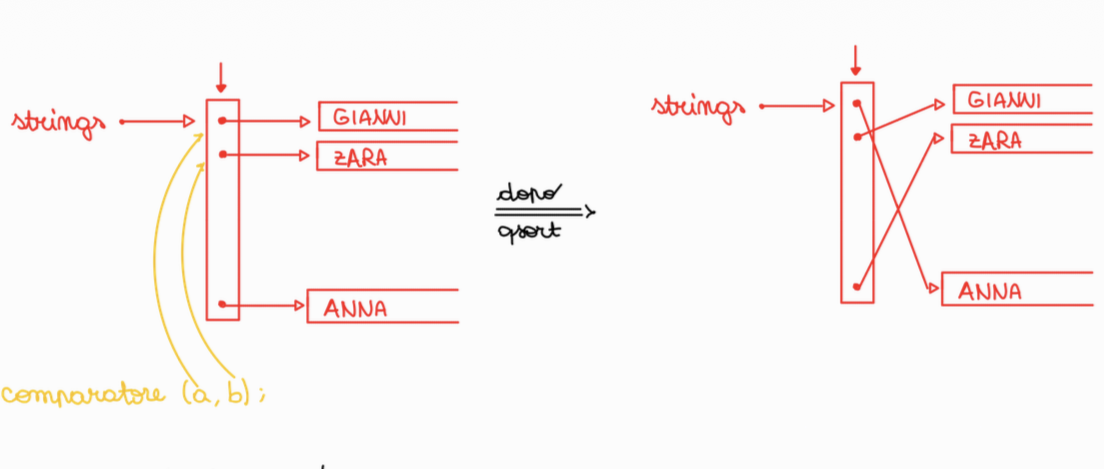
\includegraphics[width=0.8\linewidth]{../images/Qsort.png}
    \caption{Qsort}
    %\label{label}
\end{figure}
Ricordiamo che:
\begin{itemize}
    \item \texttt{p} $\rightarrow$ indirizzo
    \item \texttt{*p} $\rightarrow$ valore
    \item \texttt{\&x} $\rightarrow$ indirizzo di x
    \item \texttt{*(\&x)} $\rightarrow$ valore di x
    \item \texttt{(char **)a} $\rightarrow$ puntatore a elemento (char *)
    \item \texttt{*(char **)a} $\rightarrow$ valore di elemento (char *)
\end{itemize}
Altra funzione:
\begin{verbatim}
void bsearch (const void* key, const void *base, size_t numelem, 
             size_t sizeelem, int (*compar)(const void *, const void *));
\end{verbatim}
Cerca l'elemento \texttt{key} nell'array \textbf{\textcolor{red}{ordinato}} \texttt{base} di \texttt{numelem} elementi, ciascuno di dimensione \texttt{sizeelem}, utilizzando la funzione di confronto \texttt{compar}.
Restituisce un puntatore all'elemento trovato o \texttt{NULL} se l'elemento non è presente nell'array.\\
\textbf{\textcolor{red}{ATTENZIONE:}} l'array base deve essere ordinato poichè è una ricerca binaria.\\
Esempio di utilizzo:
\begin{verbatim}
int comparatore(const void *a, const void *b){
    int x = *(int *)a;
    int y = *(int *)b;
    return x - y;   // confronto tra due interi
}
int search_int(int v[], size_t n, int x){
    void * risultato = bsearch( &x, v, n, sizeof(int), comparatore);    
    // &x poichè devo passare un puntatore
    return risultato != NULL;
}
\end{verbatim}
\subsection{Funzioni Matematiche}
Vediamo ora le funzioni matematiche presenti nella libreria \textbf{math.h}, hanno tutte la stessa sintassi:
\begin{verbatim}
double sqrt(double x);          // restituisce la radice quadrata di x
double pow(double x, double y); // restituisce x elevato alla potenza y
double sin(double x);           // restituisce il seno di x (x in radianti)
double cos(double x);           // restituisce il coseno di x (x in radianti)
double tan(double x);           // restituisce la tangente di x (x in radianti)
double log(double x);           // restituisce il logaritmo naturale di x
double exp(double x);           // restituisce e elevato alla potenza x
\end{verbatim}
\textbf{\textcolor{red}{ATTENZIONE:}} per compilare bisogna aggiungere lo switch \texttt{-lm} per linkare la libreria matematica, altrimenti si ottiene un errore di linker.\\
\subsection{Funzioni per la Gesione degli Stream}
Vediamo ora le funzioni per la gestione degli stream presenti nella libreria \textbf{stdio.h}.Gli stream sono un astrazione
che rappresenta un flusso di byte, che può essere utilizzato per leggere o scrivere dati. Gli stream possono essere associati a file, 
dispositivi di input/output, o anche a stringhe in memoria.\\
Quando eseguiamo un programma in C, il sistema operativo assegna al corrispondente
processo automaticamente tre stream standard:
\begin{itemize}
    \item \texttt{stdin} $\rightarrow$ stream standard di input, associato alla tastiera. Utilizzato per leggere l'input del programma.
    \item \texttt{stdout} $\rightarrow$ stream standard di output, associato al terminale (schermo), utilizzato per scrivere l'output del programma.
    \item \texttt{stderr} $\rightarrow$ stream standard di errori, associato al terminale (schermo), utilizzato per scrivere messaggi di errore.
\end{itemize}
\begin{figure}[H]
    \centering  
    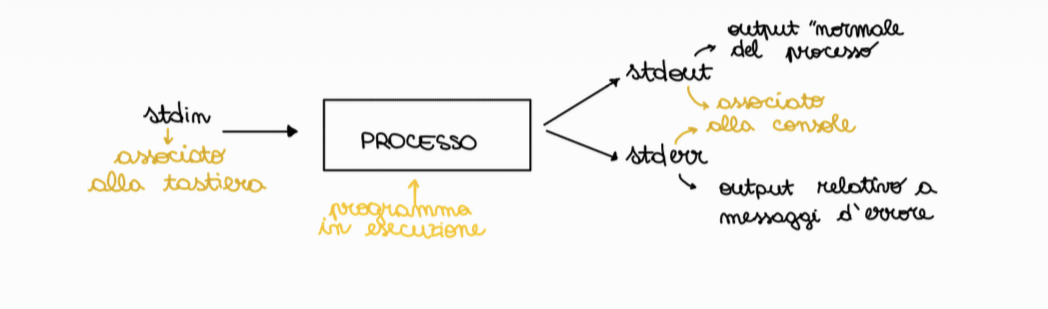
\includegraphics[width=0.9\linewidth]{../images/Gestione Stream.png}
    \caption{Stream standard}
    %\label{label}
\end{figure}
\textbf{Redirezione stdout:} è possibile redirigere l'output di un programma verso un file invece che verso il terminale, utilizzando l'operatore \texttt{>} in bash:
\begin{verbatim}
$ ./programma > output.txt
\end{verbatim}
In questo modo, l'output del programma verrà scritto nel file \texttt{output.txt} invece che sul terminale.\\
\textbf{Redirezione stderr:} è possibile redirigere anche l'output di errori verso un file, utilizzando l'operatore \texttt{2>} in bash:
\begin{verbatim}
$ ./programma 2> error.txt
\end{verbatim}
In questo modo, i messaggi di errore del programma verranno scritti nel file
\texttt{error.txt} invece che sul terminale.\\
\textbf{Redirezione stdin:} è possibile redirigere l'input di un programma da un file invece che dalla tastiera, utilizzando l'operatore \texttt{<} in bash:
\begin{verbatim}
$ ./programma < input.txt
\end{verbatim}
In questo modo, l'input del programma verrà letto dal file \texttt{input.txt} invece che dalla tastiera.\\
\textbf{Redirezione combinata:} è possibile redirigere sia l'output che l'input di un programma, utilizzando entrambi gli operatori:
\begin{verbatim}
$ ./programma < input.txt > output.txt
\end{verbatim}
In questo modo, l'input del programma verrà letto dal file \texttt{input.txt} e l'output verrà scritto nel file \texttt{output.txt}.\\
Per gestire gli stream da codice ho due opzioni:
\begin{itemize}
    \item utilizzo le libc
    \item utilizzo le syscall POSIX
\end{itemize}
Le libc sono più semplici da utilizzare, ma le syscall POSIX sono più efficienti. 
Vediamo ora le funzioni per la gestione degli stream presenti nella libreria \textbf{stdio.h}:
\begin{verbatim}
FILE *fopen(const char *path, const char *mode); // apre un file e restituisce un puntatore 
                        |                    |      di tipo FILE
                        |                    |
                        |                    |____ mode è una stringa che rappresenta le operazioni 
                        |                         da svolgere sul file: 
                        |                          r -> leggi, w -> scrivi, a -> aggiungi
                        |
                        |_____ percorso sul file system (disco) attraverso cui raggiungere il file
                               Esempio: "/home/studente/a.txt"       

int ferrore(FILE *f); // restituisce un valore diverso da 0 
                         se si è verificato un errore durante l'operazione di I/O su f
                        
void clearerr(FILE *f) // pone pari a 0 il flagi di errore

int fclose(FILE *stream); // chiude lo stream associato al file

int fprintf(FILE *stream, const char *format, ...); // scrive su stream una stringa formattata

int fscanf(FILE *stream, const char *format, ...); // legge da stream una stringa formattata



char *fgets(char *str, int n, FILE *stream); // legge da stream una stringa di al massimo n-1 caratteri 
                                            e la salva in str.  Restituisce str in caso di successo,
                                            e NULL in caso di errore o fine file

int feof(FILE *f); // restituisce un valore diverso da 0 se si è raggiunta la fine del file 

size_t fread(void *ptr, size_t size, size_t numitems, FILE *f); // legge da 'f' 'numitems' blocchi di 
                                                                elementi da leggere di
                                                                dimensione 'size' e 
                                                                li salva in 'ptr'. 
                                                                Restituisce il numero di elementi 
                                                                letti con successo

size_t fwrite(const void *ptr, size_t size, size_t numitems, FILE *f); // scrive su 'f' 'numitems' 
                                                                    blocchi di 
                                                                    elementi da scrivere di
                                                                    dimensione 'size' e 
                                                                    li legge da 'ptr'. 
                                                                    Restituisce il numero di elementi 
                                                                    scritti con successo.

int fseek(FILE *f, long offset, int whence); // sposta il puntatore al prossimo byte da 
                        |             |         leggere/scrivere in 'f'
                        |             |   
                        |             |
                        |             |________ SEEK_SET -> inizio del file
                        |                       SEEK_CUR -> posizione attuale
                        |                       SEEK_END -> fine del file
                        |
                        |_____ spostamento da applicare al puntatore espresso in byte
                                rispoetto alla posizione indicata da 'whence'         
\end{verbatim}
Esempi per capire meglio \textbf{fseek}:
\begin{verbatim}
fseek(f,10,SEEK_CUR); // sposta il puntatore di 10 byte in avanti rispetto alla posizione attuale
fseek(f,5,SEEK_SET); // sposta il puntatore al 5 byte dall'inizio del file
fseek(f,-2,SEEK_END); // sposta il puntatore a 2 byte prima della fine del file
\end{verbatim}
Continuiamo con l'ultima funzione:
\begin{verbatim}
long ftell(FILE *f); // restituisce la posizione attuale del puntatore 
                        in byte rispetto all'inizio del file
\end{verbatim}
\textbf{\textcolor{red}{ATTENZIONE:}} bisogna sempre ricordarsi di effettuare i controlli di errore su tutte queste funzioni, 
poichè possono fallire per vari motivi (file non esistente, permessi insufficienti, ecc...).\\
Vediamo qualche esempio di utilizzo:
\begin{verbatim}
// La funzione read_file deve allocare dinamicamente un buffer
// e caricarci dentro il contenuti di un file
int read_file(char *filename, void **buffer, size_t *size){
    FILE *fd = NULL;
    int res;
    long len;
    *buffer = NULL;

    fd = fopen(filename, "r");
    if(fd == NULL) goto cleanup;

    res = fseek(fd, 0, SEEK_END); // sposto il puntatore alla fine del file
    if(res == -1) goto cleanup;

    len = ftell(fd); // ottengo la lunghezza del file
    if(len == -1) goto cleanup;
    *size = (size_t)len; // salvo la lunghezza del file in size
    
    *buffer = malloc(len); // alloco un buffer di dimensione len
    if(*buffer == NULL) goto cleanup;

    res = fseek(fd, 0, SEEK_SET); // sposto il puntatore all'inizio del file
    if(res == -1) goto cleanup;

    res = fread(*buffer, 1, *size, fd); // leggo il contenuto del file nel buffer
    if(res != *size) goto cleanup; // controllo che abbia letto tutto il file

    res = fclose(fd); // chiudo il file
    if(res == -1) goto cleanup;
    return 0; // successo

    cleanup:
    int old_errno = errno; // salvo il valore di errno prima di effettuare le operazioni di pulizia
    if(fd != NULL) fclose(fd);
    if(*buffer != NULL) free(*buffer);
    errno = old_errno; // ripristino il valore di errno prima di restituire l'errore
    return -1;
}
\end{verbatim}
Passiamo ora alle syscall POSIX per la gestione degli stream, che sono più efficienti ma anche più complesse da utilizzare:
\begin{verbatim}
#include <fcntl.h>
int open(const char *pathname, int flags, mode_t mode); // apre un file e restituisce 
                        |           |       |              un file descriptor
                        |           |       |____ mode è un intero che rappresenta i permessi 
                        |           |             del file (solo se si usa O_CREAT)
                        |           |_________ flags è un intero che rappresenta la modalità di 
                        |                      apertura del file:
                        |                      O_RDONLY -> leggi, O_TRUNC -> tronca il file a 0 byte
                        |                      O_CREAT -> crea il file se non esiste
                        |                     
                        |                         
                        |_____ percorso sul file system (disco) attraverso cui raggiungere il file
                               Esempio: "/home/studente/a.txt"
\end{verbatim}
\textbf{\textcolor{red}{ATTENZIONE:}} la funzione open restituisce un file descriptor, che è un intero che rappresenta il file aperto. 
Il file descriptor 0 è riservato per stdin, 1 per stdout e 2 per stderr. I file descriptor restituiti da open sono sempre maggiori o uguali a 3.\\
Esempio di utilizzo:
\begin{verbatim}
int fd = open("file.txt",O_CREAT|O_RDONLY|O_TRUNC, 0644); // apre il file file.txt in modalità lettura 
                                                            e scrittura, se il file non esiste 
                                                            lo crea, se esiste lo tronca a 0 byte
\end{verbatim}
Abbiamo inoltre una funzione apposita per la scrittura e lettura:
\begin{verbatim}
ssize_t write(int fd, const void *buf, size_t count); // scrive su 'fd' 'count' byte da buf. 
                                                        Restituisce il numero di byte scritti 
                                                        con successo

ssize_t read(int fd, void *buf, size_t count); // legge da 'fd' 'count' byte

off_t lseek(int fd, off_t offset, int whence); // Invece di ftell si può usare
                                                  lseek(fd, 0, SEEK_CUR) per ottenere 
                                                  la posizione attuale del file descriptor
\end{verbatim}
\newpage
\section{Esecuzione dei programmi}
\subsection{Processi}
Un processo è un'istanza di un programma in esecuzione. Ogni processo ha un proprio spazio di 
indirizzamento, che include il codice del programma, i dati, lo stack e l'heap. Ogni processo ha anche un proprio stato, che può essere:
\begin{itemize}
    \item \textbf{Running} $\rightarrow$ il processo è in esecuzione
    \item \textbf{Ready} $\rightarrow$ il processo è pronto per essere eseguito, ma non è ancora stato assegnato a una CPU
    \item \textbf{Blocked} $\rightarrow$ il processo è in attesa di un evento (ad esempio, l'input dell'utente o la fine di un'operazione di I/O)
    \item \textbf{Terminated} $\rightarrow$ il processo ha terminato la sua esecuzione
\end{itemize}
Più istante dello stesso programma in \texttt{esecuzione concorrente}, ovvero che nel mentre è già in esecuzione un processo, ne viene avviato un altro che esegue lo stesso programma; 
sono rappresentate da processi distinti, con spazi di indirizzamento separati, e possono essere eseguiti in parallelo su più CPU o in modo interleaved su una singola CPU.
\begin{figure}[H]
    \centering  
    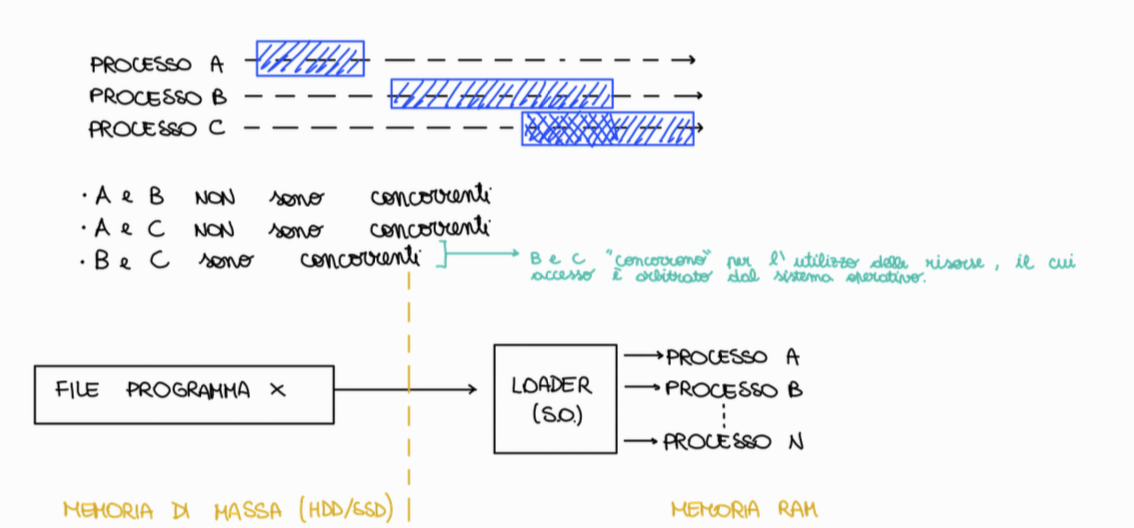
\includegraphics[width=0.9\linewidth]{../images/Interleaved 2.png}
    \caption{Programmi in esecuzione concorrente}
    %\label{label}
\end{figure}
\noindent In questo esempio B e C sono due processi concorrenti, ovvero "concorrono" per l'utilizzo delle risorse, il cui accesso è gestito dal sistema operativo. \medskip\\
\noindent Nei processi abbiamo la presenza del \textbf{Loader}, che prepara la memoria al fine di eseguire il processo, caricando il codice del programma, i dati, lo stack e l'heap. 
Il loader è responsabile anche di risolvere le dipendenze dinamiche (ad esempio, le librerie condivise) e di inizializzare il processo prima di avviarlo.
\\ Un processo è costituito dai seguenti elementi informativi:
\begin{itemize}
    \item \texttt{Immagine di Memoria} $\rightarrow$ contiene il codice del programma, i dati definiti dal programmatore, lo stack, l'heap, ecc\dots
    \item \texttt{Stato della CPU} $\rightarrow$ indica se il processo è in esecuzione, pronto, bloccato o terminato. Contiene quindi registri, ecc\dots
    \item \texttt{Risorse in uso} $\rightarrow$ indica le risorse che il processo sta utilizzando, come file aperti, socket, ecc\dots
    \item \texttt{Metadati} $\rightarrow$ contiene informazioni sul processo, come il PID (Process ID), il PPID (Parent Process ID), la priorità, 
    user, ora di avvio, linea di comando, ecc\dots. Questi metadati si possono trovare nel \textit{file system}
    all'interno di una directory speciale chiamata \texttt{/proc}, che contiene un file per ogni processo in esecuzione, con il nome del file 
    corrispondente al PID del processo. Ad esempio, il file \texttt{/proc/1234} contiene i metadati del processo con PID 1234.
\end{itemize}
\begin{figure}[H]
    \centering  
    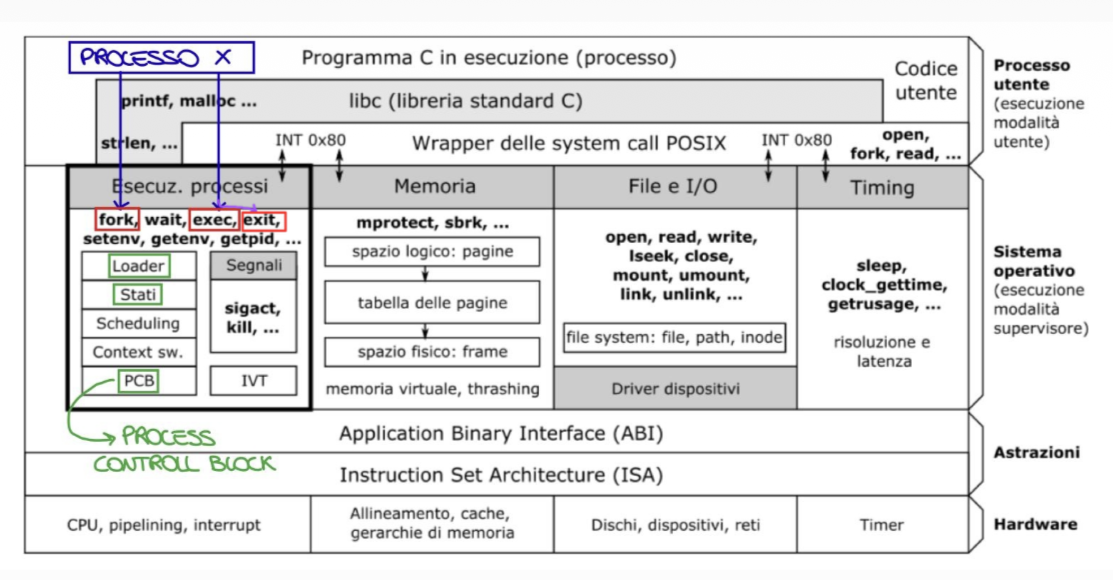
\includegraphics[width=0.9\linewidth]{../images/Processi Funzionamento yea.png}
    \caption{Processi Funzionamento}
    %\label{label}
\end{figure}
\noindent I processi per lavorare nella loro immagine di memoria non accedono direttamente
alla memoria fisica (RAM), ma utilizzano un meccanismo chiamato \textbf{memoria virtuale}, gestita dal sistema operativo;
che permette di mappare la memoria virtuale del processo alla memoria fisica del sistema. 
\begin{figure}[H]
    \centering  
    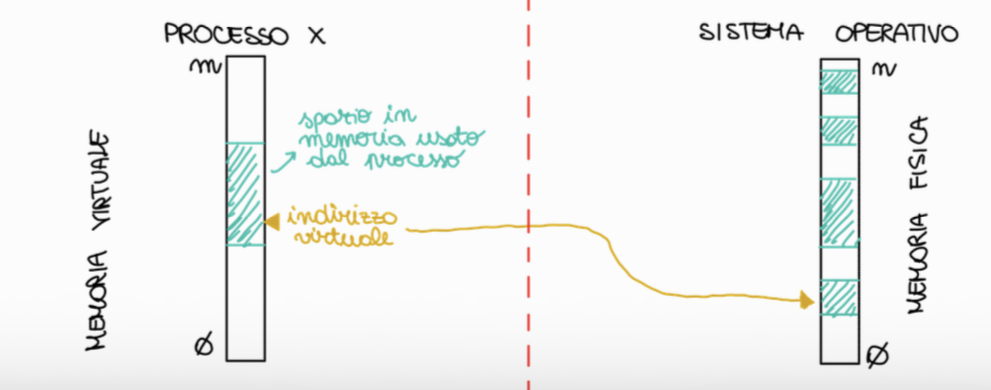
\includegraphics[width=0.9\linewidth]{../images/Memoria Virtuale.png}
    \caption{Memoria Virtuale}
    %\label{label}
\end{figure}
\noindent Consideriamo come è organizzata l'immagine di memoria di un processo dopo il caricamento di un file eseguibile (ad esempio in formato ELF).
Ogni processo vede il proprio spazio di memoria come un array lineare di byte, i cui indirizzi partono da 0 e arrivano fino a $2^b - 1$, dove $b$ rappresenta il numero di bit utilizzati per i puntatori (tipicamente 32 o 64).
I sistemi operativi garantiscono l'isolamento tra i processi attraverso il meccanismo della \textit{memoria virtuale}. Questo impedisce a un processo di accedere allo spazio di memoria di un altro processo, sia in modo malevolo 
sia a causa di errori di programmazione (bug).
\begin{figure}[H]
    \centering  
    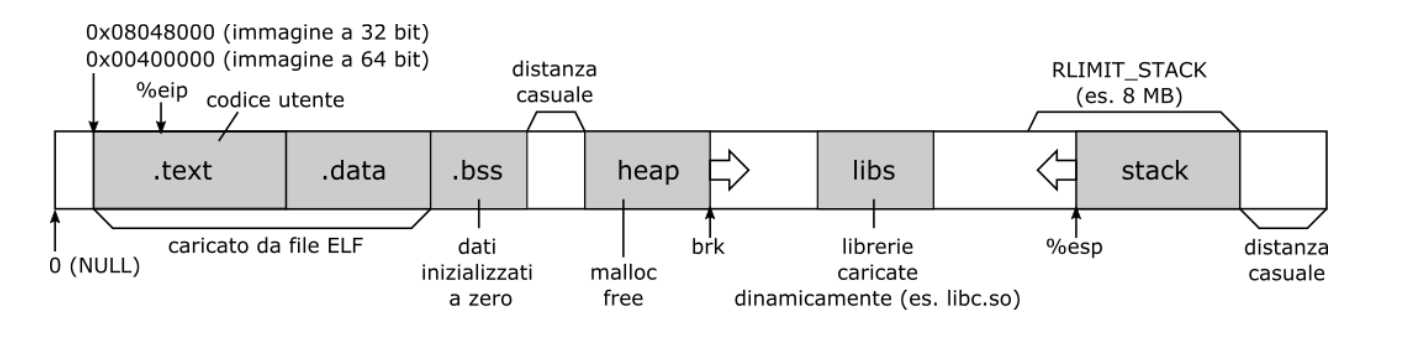
\includegraphics[width=0.9\linewidth]{../images/Immagine Processo.png}
    \caption{Immagine di un Processo}
    %\label{label}
\end{figure}
\noindent Imaginiamo di avere un codice del tipo:
\begin{verbatim}
int i[10000],  j = 10;
int main(int argc, char *argv[]){
    static char *k = "hello";
    char *p = malloc(sizeof(int) * 10000); // alloca un array di 10000 interi nell'heap
    free(p);
    printf(...);
}
\end{verbatim}
Immaginando di eseguire questo programma, l'immagine di memoria del processo sarà organizzata in questo modo:
\begin{itemize}
    \item \textbf{i} $\rightarrow$ si trova in \texttt{.bss} poiché è un array globale non inizializzato
    \item \textbf{j} $\rightarrow$ si trova in \texttt{.data} poiché è una variabile globale inizializzata
    \item \textbf{k} $\rightarrow$ si trova in \texttt{.data} poiché è una variabile statica inizializzata
    \item \textbf{"hello"} $\rightarrow$ si trova in \texttt{.rodata} poiché è una stringa letterale (read-only)
    \item \textbf{p} $\rightarrow$ la variabile si trova nello stack, mentre la memoria allocata con \texttt{malloc} si trova nell'heap
    \item \textbf{main} $\rightarrow$ si trova in \texttt{.text} poiché è codice eseguibile
    \item \textbf{argc} e \textbf{argv} $\rightarrow$ si trovano nello stack poiché sono parametri della funzione \texttt{main}
\end{itemize}
\section{Multiprogrammazione}
La \texttt{multiprogrammazione} è una tecnica che permette ai programmi di avere più processi residenti in memoria contemporaneamente, condividendo le risorse del sistema (CPU, memoria, I/O).\\
Il sistema operativo per gestire le multiple richieste di accesso alla CPU da parte dei processi concorrenti utilizza un sistema di \textbf{Time-Sharing}. Nel \texttt{Time-Sharing} tutti i processi sono "sospesi" fino a quando
non gli viene assegnato dal Sistema Operativo l'uso della CPU per un intervallo di tempo (\textbf{time slice}) durante il quale possono eseguire. Al termine del time slice, il processo 
viene nuovamente sospeso e viene assegnato un nuovo time slice a un altro processo, e così via in modo ciclico.\\
Gli stati pricnipali di un processo in un sistema multiprogrammato sono in genere tre:
\begin{itemize}
    \item \textbf{ready} $\rightarrow$ il processo è pronto per l'esecuzione, ma è tenuto fermo poiché tutti i core 
    della CPU disponibili sono impegnati nell'esecuzione di altri processi;
    \item \textbf{running} $\rightarrow$ il processo è attualmente in esecuzione su un core della CPU;
    \item \textbf{waiting/sleeping} $\rightarrow$ il processo è in attesa di un evento, come il completamento di un'operazione di I/O. Ad esempio, un processo entra nello stato waiting quando esegue una chiamata a sistema 
    che richiede la lettura di un blocco di dati da disco. Quando un processo entra in stato waiting, libera il core su cui era in esecuzione in modo che diventi disponibile per un altro processo ready.
\end{itemize}
\noindent Un processo entra tipicamente nello stato di \textit{attesa} (\textit{waiting} o \textit{sleeping}) in modo volontario, eseguendo una \textit{system call} che può richiedere tempi di completamento non trascurabili, come ad esempio operazioni di accesso alla rete o al disco.
Al termine di tali operazioni, il processo viene risvegliato e passa nello stato di \textit{ready}, ovvero pronto per essere eseguito. A questo punto interviene lo \textit{scheduling}, ovvero il meccanismo con cui il sistema operativo seleziona uno dei processi nello stato \textit{ready} per assegnargli la CPU.
Nei sistemi operativi moderni è presente il meccanismo di \textbf{preemption}, che consente di interrompere l'esecuzione di un processo in stato \textit{running} per assegnare la CPU a un altro processo. Questo meccanismo è fondamentale per garantire equità nell'uso delle risorse.
In particolare, la preemption aiuta a prevenire il fenomeno della \textbf{starvation}, in cui un processo rischia di rimanere indefinitamente in attesa senza poter progredire, a causa di altri processi che monopolizzano la CPU.
La preemption è una caratteristica tipica dei sistemi operativi \textit{time-sharing}, come \textit{Linux}, \textit{macOS} e \textit{Windows}. Tali sistemi permettono di eseguire un numero di processi superiore rispetto ai core disponibili, creando l'illusione di un'esecuzione simultanea 
grazie alla rapida alternanza dei processi sulla CPU. \\
\begin{figure}[H]
    \centering  
    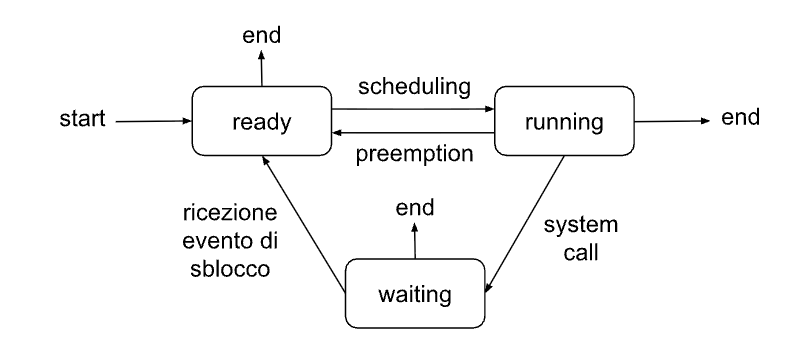
\includegraphics[width=0.6\linewidth]{../images/Stati Processi CPU.png}
    \caption{Stati dei processi e CPU}
    %\label{label}
\end{figure}
\noindent Per evitare la \texttt{starvation}, possiamo adoperare:
\begin{enumerate}
    \item \textbf{Preemption} 
    \item \textbf{Scheduler} con algoritmo di tipo \textit{fair time sharing} (esempio round-robin).
\end{enumerate}
\noindent Per consentire a tutti i processi ready di progredire uniformemente nell'esecuzione, un popolare algoritmo di 
schedulazione è il \textbf{round-robin}, che assegna un core a rotazione a ciascun processo ready per la durata di una time slice.\\
Il sistema operativo può anche implementare un sistema di \textbf{priorità} per i processi, in modo che alcuni processi vengano eseguiti più frequentemente di altri.
In pratica è spesso possibile assegnare una priorità a un processo in modo che venga schedulato per l'esecuzione più frequentemente degli altri. 
Il funzionamento dell'algoritmo di schedulazione round-robin è illustrato nel seguente diagramma a tre processi con la stessa priorità:
\begin{figure}[H]
    \centering  
    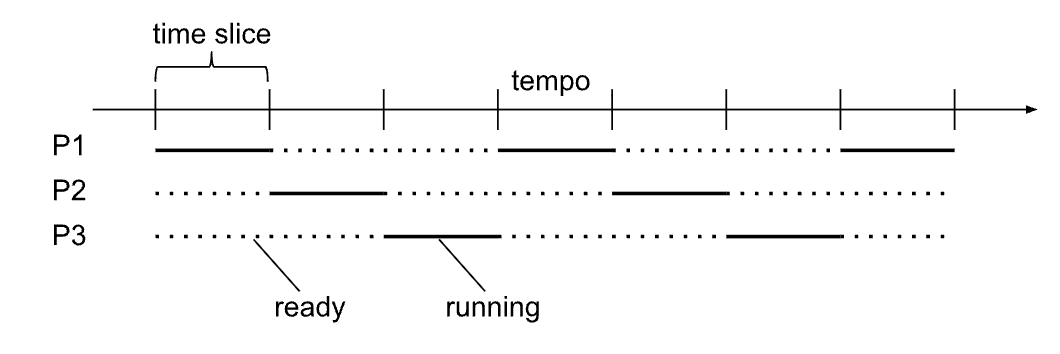
\includegraphics[width=0.7\linewidth]{../images/round-robin.png}
    \caption{Round-Robin}
    %\label{label}
\end{figure}
\noindent Come si vede, l'algoritmo round-robin non genera starvation nei processi, che hanno tutti l'opportunità di progredire nella computazione. Il sistema operativo 
tiene tipicamente i PCB dei processi organizzati in liste separate per ciascuno stato.
\subsection{Funzioni per la gestione dei processi}
Vediamo ora le funzioni per la gestione dei processi presenti nella libreria \textbf{unistd.h}:
\begin{verbatim}
fork () ->  Genera un nuovo processo (chiamato processo figlio) che è una copia del processo chiamante 
            (chiamato processo padre). Il processo figlio ha un proprio PID (Process ID) e 
            PPID (Parent Process ID), ma condivide con il processo padre lo stesso codice, dati, 
            stack e heap (inizialmente). La funzione fork restituisce 0 al processo figlio 
            e il PID del processo figlio. Una volta generata la copia del processo, vengono
            messi in stato di READY entrambi i processi (padre e figlio) e il sistema 
            operativo decide quale dei due eseguire per primo.
\end{verbatim}
\textbf{\textcolor{red}{ATTENZIONE:}} in questo momento i due processi possono essere distinti
solo perchè hanno PID diversi, ma condividono lo stesso spazio di memoria, quindi se uno dei 
due processi modifica una variabile, anche l'altro processo vedrà la modifica.
\begin{verbatim}
pid_t fork(); 
\end{verbatim}
Restituisce:
$\begin{cases}
    \textbf{-1}  \text{ in caso di errore} \\
    \textbf{0}  \text{  restituisce il PID del nuovo processo creato (figlio)} \\
    \textbf{$>$0} \text{  restituito al processo che ha invocato fork()
    (processo padre) e rappresenta il PID del processo creato}. \\
\end{cases}$
\medskip\\ \noindent Per distinguiere il codice che va eseguito nel processo padre/figlio si usa la seguente struttura:
\begin{verbatim}
#include <stdlib.h>
#include <unistd.h>
int main(){
    pid_t pid = fork();
    if(pid == -1){
        // gestione errore
        exit(-1);   
    } else if(pid == 0){
        // codice eseguito dal processo figlio
        printf("sono il processo figlio\n");
    } else {
        // codice eseguito dal processo padre
        printf("sono il processo padre\n");
    }
    return 0;
}
\end{verbatim}
Vediamo ora \textbf{Fork Multiple}:
\begin{verbatim}
int main(){
    pid_t p1 = fork();
    pid_t p2 = fork();
    pid_t p3 = fork();
    // In totale si ottengono 8 processi (2^3)
    if(p3 == 0){
        // eseguito dai processi figli dell'ultima fork()
        printf("*");
        // 4 processi stampano "*"
    } else if(p2 == 0){
        // eseguito dai processi che sono figli della seconda fork()
        // ma NON figli della terza
        printf("+");
        // 2 processi stampano "+"
    } else if(p1 == 0){
        // eseguito dai processi che sono figli della prima fork()
        // ma NON figli della seconda e terza
        printf("-");
        // 1 processo stampa "-"
    } else {
        // processo padre originale (non figlio di nessuna fork)
        printf("0");
        // 1 processo stampa "0"
    }
}
\end{verbatim}
\begin{figure}[H]
    \centering  
    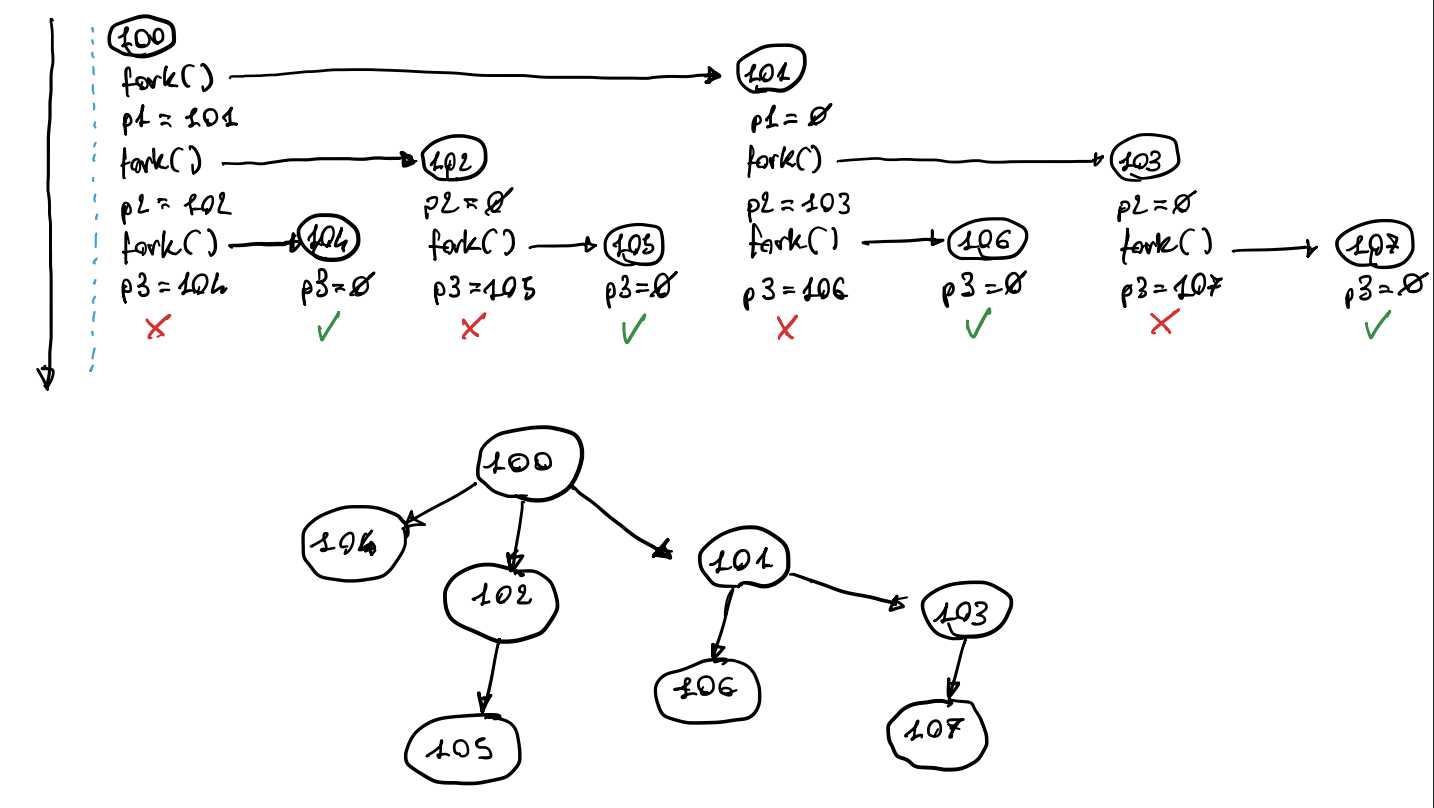
\includegraphics[width=0.8\linewidth]{../images/Esempio Fork Multipli .png}
    \caption{Fork Multipli}
    %\label{label}
\end{figure}
Quale codice genera il seguente albero di processi?
\begin{figure}[H]
    \centering  
    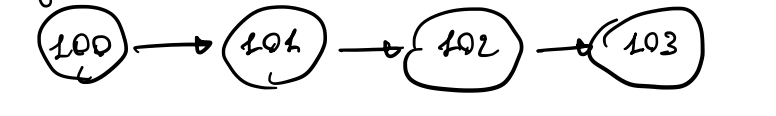
\includegraphics[width=0.8\linewidth]{../images/Albero Fork .png}
    \caption{Fork Multipli}
    %\label{label}
\end{figure}
\begin{verbatim}
int main(){
    pid_t p1 = fork();
    if(p1 == 0) pid_t p2 = fork();
    if(p2 == 0) pid_t p3 = fork();
    if(p3 == 0) printf("*");
    // abbiamo 1 solo processo che stampa * dato che solo 1 processo
    // avrà come padre p3 e quindi eseguirà il codice che stampa "*"
}
\end{verbatim}
FARE ESERCIZIO !="£="£=")£"=£"\\
Altri comandi utili:
\begin{verbatim}
pid_t getpid();     -> restituisce il PID del processo chiamante (PID processo figlio)
pid_t getppid();    -> restituisce il PPID del processo chiamante (PPID processo padre)
_exit(int status);  -> funziona come exit() ma non esegue l'eventuale gestione della
                       terminazine
\end{verbatim}
\subsection{Sincronizzazione dei processi}
La sincronizzazione dei processi è un aspetto fondamentale nei sistemi operativi, poiché permette di coordinare l'accesso alle risorse condivise tra più processi concorrenti.
In un sistema multiprogrammato, più processi possono accedere contemporaneamente a risorse condivise, come ad esempio file, memoria, dispositivi di I/O, ecc\dots
Senza un meccanismo di sincronizzazione, si potrebbero verificare situazioni di \textbf{race condition}, in cui il risultato di un'operazione dipende dall'ordine di esecuzione dei processi, 
portando a comportamenti imprevedibili e potenzialmente dannosi. Il processo padre può quindi voler sapere quando i suoi processi figli terminano la loro esecuzione.\\
\textbf{\textcolor{red}{IMPORTANTE:}} non possiamo mai far alcuna assunzione sui tempi e sull'ordine con cui
verranno eseguite le istruzioni nei processi concorrenti, poiché dipende dallo scheduler del sistema operativo, che può decidere di eseguire i processi in modo interleaved o in parallelo su più CPU.
\begin{verbatim}
#include <sys/types.h>
#include <sys/wait.h>
pid_t wait(int *status);    ->  restisce il PID del processo figlio che è terminato, e salva lo stato 
                                di terminazione del processo figlio in status. 
                                Se non ci sono processi figli, restituisce -1. Wait è bloccante 
                                fino alla terminazione di un processo figlio.
\end{verbatim}
Quando invoco wait sono possibili due casi:
\begin{enumerate}
    \item \textbf{Il processo figlio è già terminato} $\rightarrow$ in questo caso wait restituisce immediatamente il PID 
    del processo figlio terminato e lo stato di terminazione.
    \item \textbf{Il processo figlio non è ancora terminato} $\rightarrow$ in questo caso wait rimane bloccato fino 
    a quando il processo figlio non termina, momento in cui restituisce il PID del processo figlio terminato e lo stato di terminazione.
\end{enumerate}
\textbf{\textcolor{red}{ATTENZIONE:}} se il processo padre termina prima del processo figlio, il processo figlio diventa un processo \textit{orfano} 
e viene adottato dal processo \texttt{init} (PID 1), che si occupa di gestire i processi orfani.\\
Per leggere il valore di uscita del processo figlio, possiamo utilizzare le seguenti macro:
\begin{verbatim}
wifextied(status_ptr) ->    restituisce il valore 1 se il processo figlio è terminato normalmente 
                            (ad esempio, chiamando exit() o return dalla funzione main)
                             altrimenti restituisce 0
wexitstatus(status_ptr) ->  restituisce il codice di terminaazione ottenuto dal figlio
\end{verbatim}
\subsection{Caricamento di programmi}
Il caricamento di un programma è il processo mediante il quale un file eseguibile viene caricato in memoria e preparato per l'esecuzione.
\begin{verbatim}
#include <unistd.h>
int execvp(const char *filename, char *argv[]);
|               |                      |                               
|               |                      |_____ array di stringhe terminato con NULL che contiene gli  
|               |                             argomentida passare al main del programma, 
|               |                             dove argv[0] deve essere il nome del programma eseguibile.
|               |
|               |____ percorso su disco del programma           
|                     da eseguire (esempio: "/bin/ls")          
|                                                               
|____ restituisce - 1 in caso di errore
\end{verbatim}
execvp sostituisce integralmente l'immagine di memoria del processo che la invoca con quella del
programma da eseguire:
\begin{figure}[H]
    \centering  
    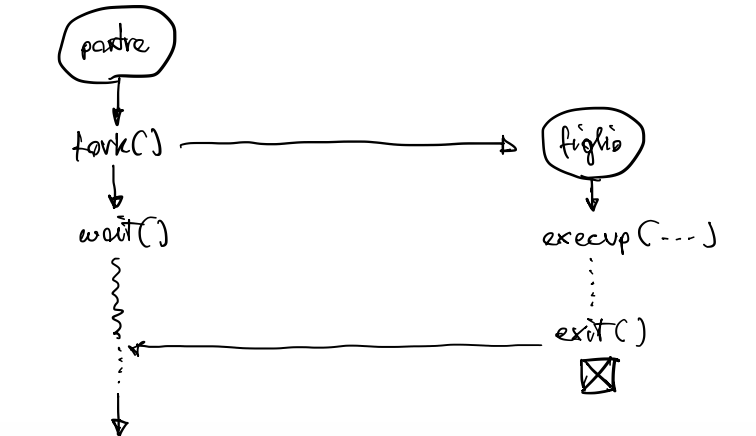
\includegraphics[width=0.7\linewidth]{../images/execvp.png}
    \caption{Esecuzione di un programma con execvp}
    %\label{label}
\end{figure}
\begin{verbatim}
int main(){
    if(pid == -1){
        perror("fork");
        return EXIT_FAILURE;
    }
    if(pid == 0){
        char* argv[] = {"ls", "-l", NULL};
        execvp("ls", argv); 
        perror("execvp");
        _exit(EXIT_FAILURE);
    }
    return EXIT_SUCCESS;
}
\end{verbatim}
\newpage
\section{Thread}
I thread nascono per ridurre il costo computazionale (\textit{overhead}) dovuto alla multiprogrammazione.  
Un processo può essere composto da una o più unità di esecuzione chiamate \texttt{thread}.\\
Un \textbf{thread} è un'unità di esecuzione più leggera rispetto a un processo.  
I thread appartenenti allo stesso processo condividono:
\begin{itemize}
    \item lo stesso codice del programma;
    \item la gran parte dei dati in memoria (costanti, variabili globali,
    variabili statiche, heap, ecc\dots);
    \item file aperti;
    \item segnali e le loro routine di gestione;
    \item directory di lavoro corrente;
    \item diritti dell'utente proprietario del processo;
    \item lo stesso spazio di memoria;
    \item le stesse risorse del processo padre;
\end{itemize}
Ovvero la \texttt{sezione dati}, \textbf{\textcolor{red}{TUTTI}} i thread associati ad uno stesso processo ne condividono l'immagine di memoria.\\
Grazie a questa condivisione, i thread possono collaborare ed eseguire più attività contemporaneamente 
all'interno dello stesso processo, migliorando efficienza e reattività del programma.\\
In pratica, un thread può essere visto come una sequenza di istruzioni che viene 
eseguita in modo indipendente rispetto agli altri thread dello stesso programma.\\
Ciascun thread gestisce in modo indipendente le seguenti informazioni:
\begin{enumerate}
   \item Un identificatore univoco \textbf{(Thread ID)};
   \item \textbf{Stack}
   \item \textbf{Stato} della CPU (registri, IP, ecc\dots)
   \item alcune variabili \textbf{globali} (ad esempio, errno)
   \item \textbf{Metadati} (proprietà specifiche di ogni thread, come priorità, stato, ecc\dots)
\end{enumerate}
\begin{figure}[H]
    \centering  
    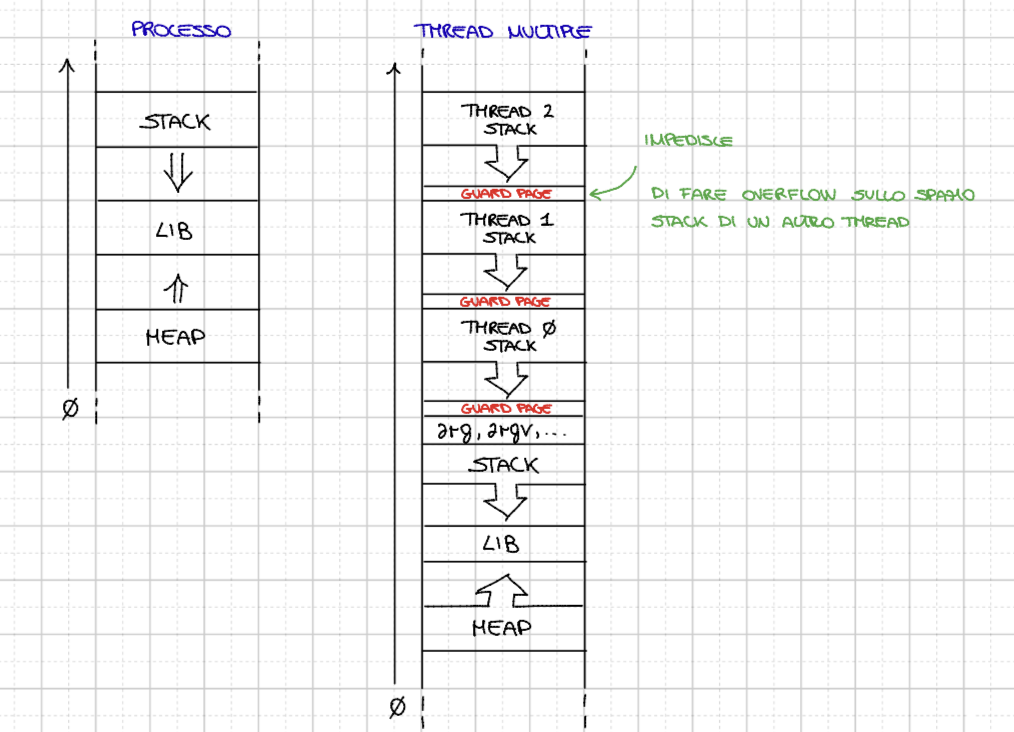
\includegraphics[width=0.85\linewidth]{../images/Thread Multipli REAL.png}
    \caption{Thread}
    %\label{label}
\end{figure}
Come possiamo vedere nei thread multipli in ogni stack il sistema operativo inserisce il \textbf{guard page} ovvero uno
spazio di memoria non accessibile che serve a rilevare eventuali overflow dello stack, evitando così che un thread possa sovrascrivere lo stack di un altro thread.\\
\textbf{\textcolor{red}{ATTENZIONE:}} se un thread va in \texttt{crash} a causa di un errore di segmentazione (ad esempio, accedendo a una posizione di memoria non valida),
tutti i thread dello stesso processo vanno in crash, poiché condividono lo stesso spazio di memoria.\\
Riassumendo:
\begin{enumerate}
    \item Un thread esiste all'interno di un processo e ne condivide le risorse;
    \item Ogni thread ha un controllo del flusso di esecuzione del codice indipendentemente dagli altri;
    \item Un thread duplica le risorse minime necessarie per il suo funzionamento;
    \item Un thread condivide le risorse del processo con gli altri thread dello stesso processo;
\end{enumerate}

\subsection{Posix Thread}
I Posix Thread (Pthread) sono una specifica standard per la gestione dei thread nei sistemi operativi Unix-like.\\
\textbf{\textcolor{red}{IMPORTANTE}}: per usaere i posix thread bisogna compilare con switch "-lpthread" per linkare la libreria pthread.\\
\noindent Vediamo una prima funzione di \texttt{pthread.h}:
\begin{verbatim}
#include <pthread.h>
int pthread_create(pthread *threadID, const pthread_attr_t *attr, 
                    void *(*start_routine)(void *), void *arg);
\end{verbatim}
Questa funzione restituisce 0 in caso di successo, altrimenti restituisce un codice di errore, mentre per quanto riguarda i parametri:
\begin{itemize}
    \item \textbf{pthread *threadID} $\rightarrow$ puntatore a una variabile di tipo pthread che in caso
    di successo contiene l'identificatore del thread creato
    \item \textbf{const pthread\_attr\_t *attr} $\rightarrow$ struct con cui specificare attributi del thread
    \item \textbf{void *(*start\_routine)(void *)} $\rightarrow$ puntatore alla funzione che il thread dovrà eseguire
    \item \textbf{void *arg} $\rightarrow$ eventuali parametri per la funzione eseguita nel thread
\end{itemize}
Nei thread la funzione exit non è la funzione giusta da utilizzare, ma dovremmo usare:
\begin{verbatim}
void pthread_exit(void *retval)
\end{verbatim}
L'istruzione termina il thread corrente restituendo \texttt{retval}, ovvero il parametro che abbiamo passato.
Vediamo un esempio:
\begin{verbatim}
void  *PrintHello(void *threadid){
    long tid;
    tid = (long) threadid;
    printf("Hello Word! Sono il thread #%ld!\n", tid);
    pthread_exit(NULL);
}
int main(int argc, char *argv[]){
    pthread_t threads[NUM_THREADS];
    int rc;
    long t;
    for(t = 0; t < NUM_THREADS; t++){
        printf("Funzione main: creo il thread %ld\n", t);
        rc = pthread_create(&threads[t], NULL, PrintHello, (void*) t);
        pthread_detach(threads[t]);
        if(rc){
            printf("ERRORE: codice %d\n", rc);
            exit(-1);
        }
    }
    sleep(2);
}
\end{verbatim}
\noindent Abbiamo poi:
\begin{verbatim}
int pthread_join(pthread_t threadID, void ** retval);
                        |               |
                        |               |____ puntatore a variabile in cui sarà memorizzato 
                        |                     il valore di ritorno
                        |
                        |_____ ID del thread di cui si vuole attendere
                               la terminazione
\end{verbatim}
La funzione \texttt{pthread\_join} permette a un thread di aspettare la terminazione di un altro thread esclusivamente se "joinable" al thread che li ha creati.\\
\noindent Un thread può essere:
\begin{itemize}
    \item \textbf{joinable} $\rightarrow$ il thread che lo ha creato può aspettarne la fine usando \texttt{pthread\_join};
    \item \textbf{detached} $\rightarrow$ termina in modo indipendente e nessun altro thread può aspettarlo con \texttt{pthread\_join}.
\end{itemize}
\noindent Quindi, quando un thread è \textbf{joinable}, il thread creatore può:
\begin{itemize}
    \item fermarsi in attesa della sua terminazione;
    \item recuperare il valore restituito dal thread;
    \item liberare correttamente le risorse utilizzate.
\end{itemize}
\noindent Per rendere un thread detached, si può usare la funzione:
\begin{verbatim}
int pthread_detach(pthread_t threadID);
\end{verbatim}
\textbf{\textcolor{red}{ATTENZIONE:}} se un thread è detached, non è possibile aspettarne la terminazione con \texttt{pthread\_join}. Si dice
che "distacca" il threadID dal thread che lo ha creato, rendendolo indipendente.
\noindent 
\subsection{Come la CPU esegue le istruzioni}

Fino ad ora abbiamo assunto che ogni istruzione Assembly venga eseguita in modo ``atomico''.
In realtà, all'interno della CPU, l'esecuzione di un'istruzione richiede diversi passaggi intermedi.

\begin{figure}[H]
    \centering  
    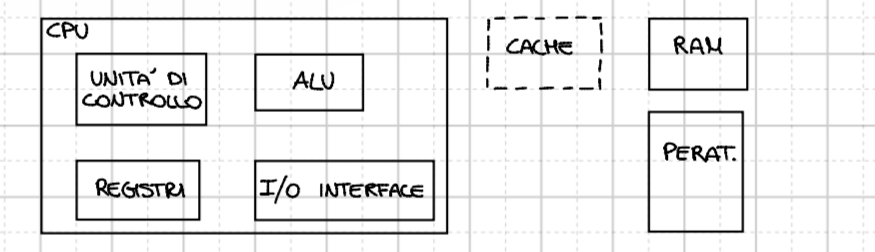
\includegraphics[width=0.9\linewidth]{../images/CPU ISTRUZIONI.png}
    \caption{CPU}
    %\label{label}
\end{figure}

\noindent
Ogni istruzione viene eseguita dalla CPU attivando, in una precisa sequenza temporale,
diversi componenti elettronici interni. 
Ciascun componente deve essere attivato nel momento corretto affinché venga rispettata
la semantica dell'istruzione.

\noindent L'attività dei vari componenti è coordinata dall'unità di controllo (\textit{Control Unit})
e deve essere accuratamente temporizzata.
L'esecuzione avviene quindi per stadi (\textit{stages}) di durata prefissata.

\noindent Supponendo di considerare una CPU RISC semplificata, l'esecuzione di un'istruzione
può essere suddivisa nelle seguenti fasi:

\begin{enumerate}
    \item \textbf{Fetch (F)} $\rightarrow$ la CPU preleva dalla memoria la prossima istruzione da eseguire. 
    Successivamente viene aggiornato il \textit{Program Counter} (PC), in modo che punti
    all'istruzione successiva.

    \item \textbf{Decode (D)} $\rightarrow$ l'istruzione appena letta viene interpretata analizzandone
    l'opcode. In questa fase vengono inoltre letti gli eventuali operandi immediati
    e i valori contenuti nei registri coinvolti.

    \item \textbf{Execute (E)} $\rightarrow$ se previsto dall'istruzione, l'ALU
    (\textit{Arithmetic Logic Unit}) esegue l'operazione richiesta e calcola il risultato.

    \item \textbf{Memory (M)} $\rightarrow$ se necessario, viene effettuato un accesso alla memoria
    in lettura o scrittura.

    \item \textbf{Write-Back (W)} $\rightarrow$ il risultato finale viene scritto nei registri
    di destinazione, se richiesto dall'istruzione.
\end{enumerate}

\begin{figure}[H]
    \centering  
    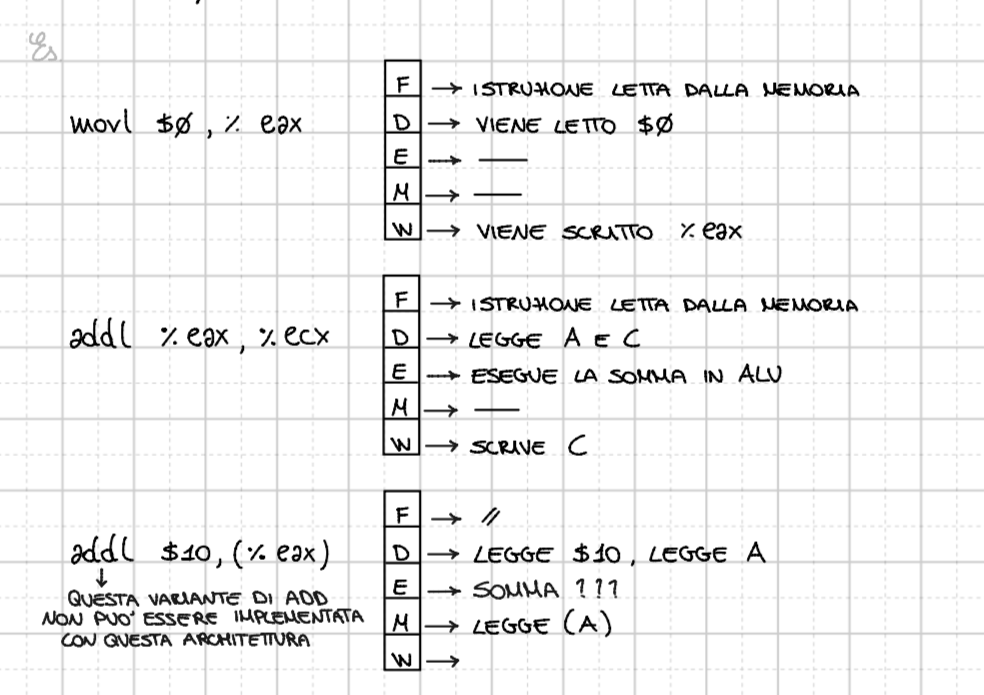
\includegraphics[width=0.9\linewidth]{../images/Esecuzione a STATI .png}
    \caption{Esempio di esecuzione a stadi}
    %\label{label}
\end{figure}

\noindent
Le architetture \textbf{RISC} (\textit{Reduced Instruction Set Computer})
semplificano l'esecuzione delle istruzioni mantenendo un numero limitato di operazioni semplici.

\begin{itemize}
    \item numero elevato di registri e istruzioni semplici;
    \item esecuzione più rapida delle istruzioni;
    \item pipeline più semplice ed efficiente;
    \item programmi generalmente più lunghi.
\end{itemize}

\noindent
Le architetture \textbf{CISC} (\textit{Complex Instruction Set Computer}),
invece, utilizzano istruzioni più complesse e potenti.
\begin{itemize}
    \item numero ridotto di istruzioni, ma più sofisticate;
    \item istruzioni spesso più lente da eseguire;
    \item hardware di controllo più complesso;
    \item programmi generalmente più compatti.
\end{itemize}
\begin{figure}[H]
    \centering  
    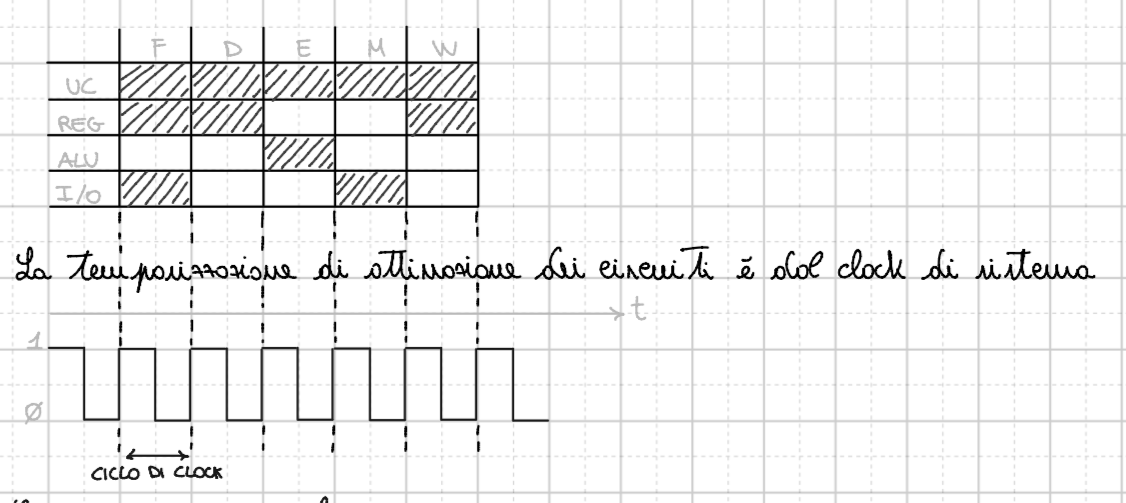
\includegraphics[width=0.9\linewidth]{../images/CISC.png}
    \caption{Graficamente}
    %\label{label}
\end{figure}
La temporizzazione di attivazione dei circuiti è dal clock di sistema.
\subsection{Esecuzione con Pipelining}
Supponiamo di dover eseguire tre istruzioni consecutive.

\begin{figure}[H]
    \centering  
    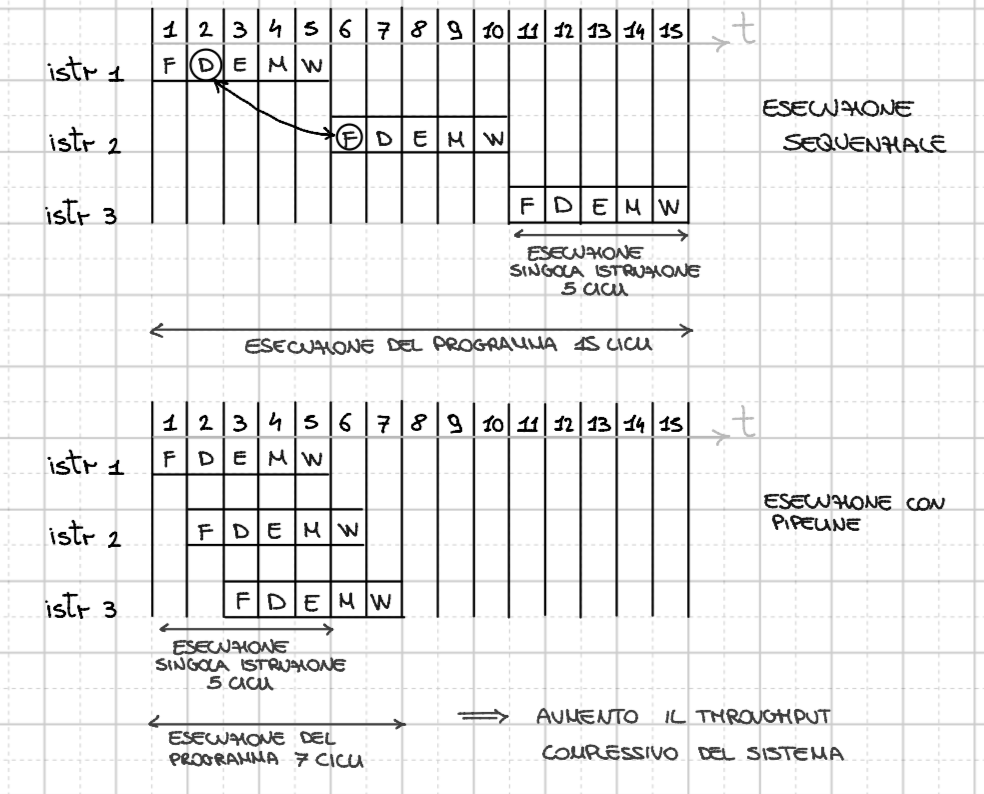
\includegraphics[width=0.9\linewidth]{../images/Pipilenie.png}
    \caption{Esempio di pipeline}
    %\label{label}
\end{figure}

\noindent
Nel \textbf{pipelining}, l'esecuzione delle istruzioni viene suddivisa in più stadi,
che possono lavorare in parallelo su istruzioni differenti.
In questo modo, mentre un'istruzione si trova in una certa fase, un'altra può trovarsi
in una fase successiva o precedente.

\medskip

\noindent
\textbf{\textcolor{red}{Attenzione:}} mantenere la pipeline sempre ``piena''
consente di massimizzare il \textit{throughput}, cioè il numero di istruzioni completate
nell'unità di tempo.

\noindent Tuttavia, non è sempre possibile occupare tutti gli stadi della pipeline a causa
della presenza degli \textbf{hazard}, ovvero situazioni che impediscono la corretta
esecuzione parallela delle istruzioni.

\subsubsection*{Hazard strutturali}

Gli \textbf{hazard strutturali} si verificano quando due o più istruzioni richiedono
contemporaneamente la stessa risorsa hardware della CPU.

\begin{figure}[H]
    \centering  
    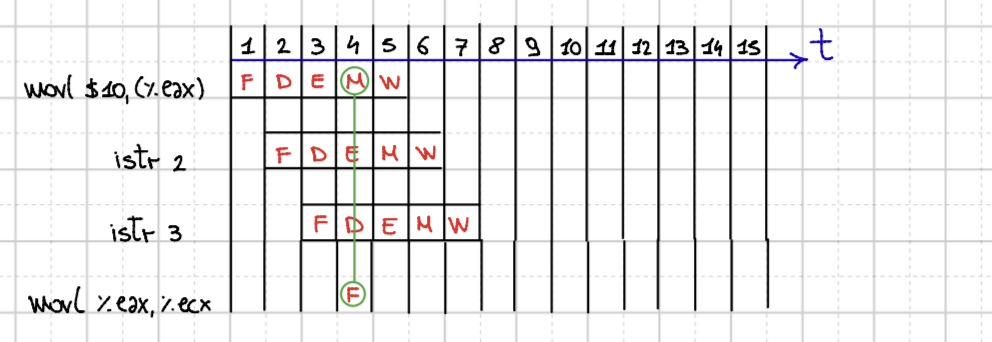
\includegraphics[width=0.9\linewidth]{../images/Hazard Strutturali.png}
    \caption{Esempio di hazard strutturale}
    %\label{label}
\end{figure}

\noindent
Possibili soluzioni:

\begin{itemize}
    \item utilizzare cache separate per dati e istruzioni;
    \item duplicare le risorse hardware coinvolte;
    \item introdurre uno \textbf{stallo} (\textit{stall}) della pipeline.
\end{itemize}

\noindent
\textbf{Tecnica dello stallo:}
la CPU blocca temporaneamente la pipeline, impedendo l'ingresso di nuove istruzioni,
per il numero minimo di cicli di clock necessario a risolvere l'hazard.

\begin{figure}[H]
    \centering  
    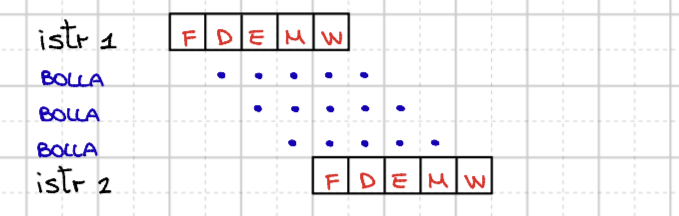
\includegraphics[width=0.9\linewidth]{../images/Stallo Pipe.png}
    \caption{Pipeline in stallo}
    %\label{label}
\end{figure}

\noindent
L'introduzione di ``bolle'' (\textit{bubbles}) nella pipeline consente di risolvere
qualsiasi hazard, ma comporta una riduzione del throughput.

\subsubsection*{Hazard sui dati}

Gli \textbf{hazard sui dati} si verificano quando esistono dipendenze tra i dati
utilizzati da istruzioni differenti.

\begin{figure}[H]
    \centering  
    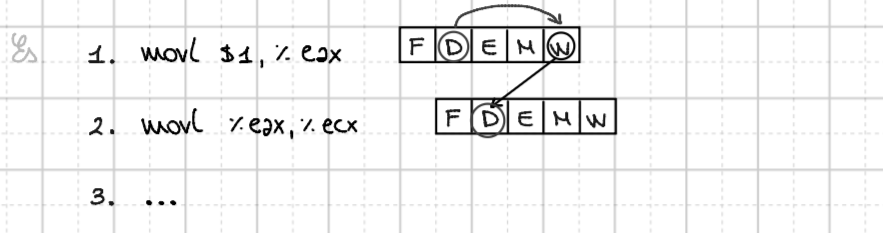
\includegraphics[width=0.9\linewidth]{../images/Hazard sui dati.png}
    \caption{Esempio di hazard sui dati}
    %\label{label}
\end{figure}

\noindent
Una possibile soluzione consiste nel \textbf{riordinamento del codice},
cioè modificare l'ordine delle istruzioni senza alterare la semantica del programma,
in modo da evitare conflitti tra i dati.

\medskip

\begin{minipage}{0.35\textwidth}
\begin{verbatim}
movl $4, %eax
movl %eax, %ecx
movl $2, %ebx
movl $3, %edi
movl $4, %esi
\end{verbatim}
\end{minipage}
\hfill
$\Longrightarrow$
\hfill
\begin{minipage}{0.35\textwidth}
\begin{verbatim}
movl $4, %eax
movl $2, %ebx
movl $3, %edi
movl $4, %esi
movl %eax, %ecx
\end{verbatim}
\end{minipage}

\medskip

\noindent
Nell'esempio precedente, l'istruzione

\begin{verbatim}
movl %eax, %ecx
\end{verbatim}

\noindent
viene spostata alla fine poiché non influenza le altre istruzioni
e può quindi essere eseguita successivamente senza modificare il comportamento del programma.

\subsubsection*{Hazard sul controllo di flusso}

Gli \textbf{hazard sul controllo di flusso} si verificano quando l'esecuzione di un'istruzione
dipende dal risultato di una precedente istruzione di salto condizionato.

\begin{verbatim}
testl %eax, %eax
je L1
movl %eax, %edx
L1:
.
.
.
\end{verbatim}

\noindent
In questo caso, la CPU non può sapere immediatamente quale sarà la prossima istruzione
da eseguire finché la condizione del salto non viene valutata.

\medskip

\noindent
\textbf{Branch Prediction:}
la CPU tenta di predire quale sarà il prossimo ramo di esecuzione,
così da continuare a riempire la pipeline senza attendere il risultato effettivo del salto.

\medskip

\noindent
\textbf{Uso di codice alternativo:}
in alcuni casi è possibile sostituire salti condizionati con istruzioni che non alterano
il flusso di controllo, riducendo così gli hazard.

\begin{verbatim}
testl %eax, %eax
cmovl %eax, %edx
\end{verbatim}

\noindent
L'istruzione \texttt{cmovl} (\textit{conditional move}) esegue il trasferimento
solo se la condizione specificata risulta verificata, evitando un salto esplicito.
\subsection{Interruzioni}

Un \textbf{interrupt} è una segnalazione generata dall'hardware oppure tramite
specifiche istruzioni software, che richiede l'attenzione immediata del sistema.

\noindent La notifica di un interrupt rappresenta un evento asincrono rispetto al normale
flusso di esecuzione del programma.
Quando si verifica un interrupt, l'esecuzione del processo nello stato
\texttt{RUNNING} viene sospesa e il processo passa tipicamente nello stato
\texttt{READY}. Successivamente, il sistema operativo esegue una particolare
routine di gestione dell'evento detta \textbf{interrupt handler}.

\medskip

\noindent
Eventi differenti vengono gestiti da handler differenti.
La corrispondenza tra interrupt e relativo handler è mantenuta dal sistema operativo
attraverso una struttura dati chiamata
\textbf{Interrupt Vector Table (IVT)}.

\begin{figure}[H]
    \centering  
    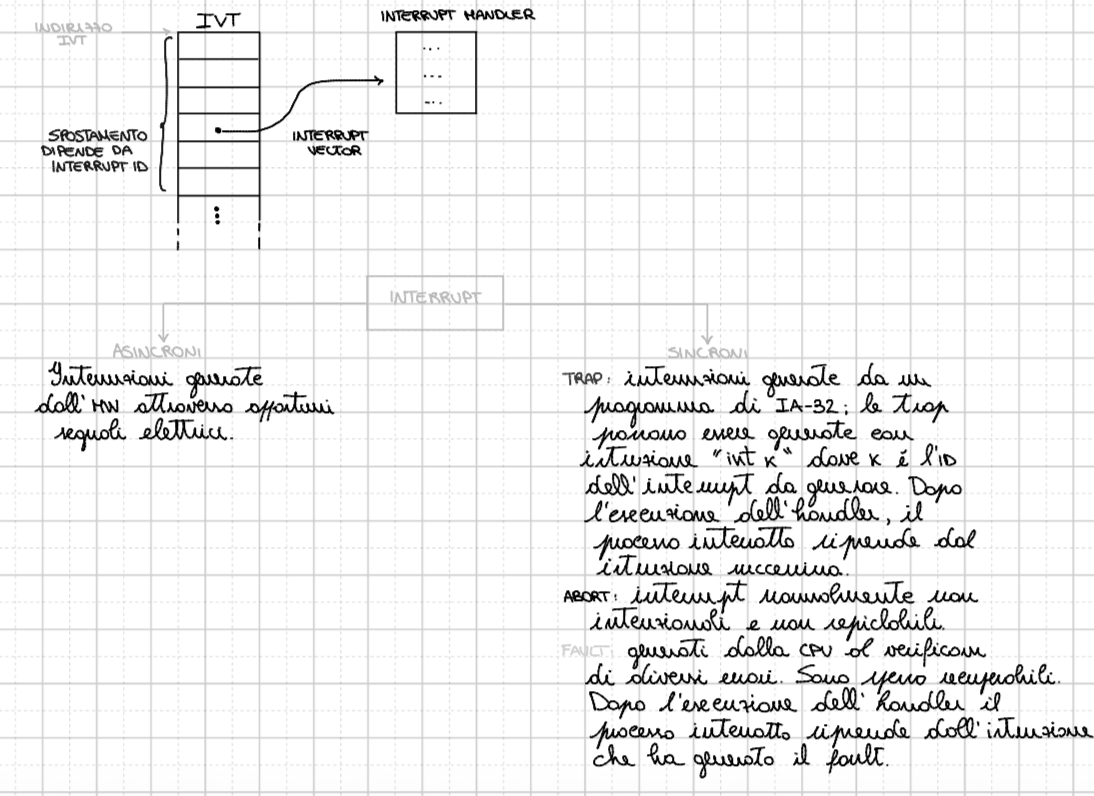
\includegraphics[width=0.9\linewidth]{../images/IVT.png}
    \caption{Interrupt Vector Table}
    %\label{label}
\end{figure}

\subsubsection*{Tipologie di interrupt}

\begin{itemize}
    \item \textbf{Abort} $\rightarrow$ interrupt generalmente non intenzionale e non recuperabile.
    Solitamente provoca la terminazione del processo corrente.

    \item \textbf{Fault} $\rightarrow$ interrupt generato dalla CPU al verificarsi di errori
    durante l'esecuzione di un'istruzione. 
    I fault sono spesso recuperabili.
    
    Dopo l'esecuzione dell'handler, il processo interrotto può riprendere
    dall'istruzione che ha generato il fault.
\end{itemize}
\newpage
\section{Segnali}

Un \textbf{segnale} è una notifica asincrona inviata a un processo per indicare il verificarsi di un evento specifico.  
I segnali vengono utilizzati dal Sistema Operativo per gestire situazioni come errori, interruzioni, eccezioni o richieste di terminazione.
Gli \textbf{interrupt}, invece, sono il meccanismo con cui l'hardware comunica al Sistema Operativo la necessità di gestire una particolare condizione.  
Dal punto di vista concettuale, interrupt e segnali svolgono un ruolo simile: notificare il verificarsi di un evento asincrono.

\medskip

\begin{table}[H]
\centering
\begin{tabular}{|l|l|l|l|}
\hline
\textbf{Meccanismo} & \textbf{Destinatario} & \textbf{Mittente} & \textbf{Gestore} \\
\hline
Interrupt & Kernel 
          & Periferiche, CPU, programmi 
          & Interrupt Handler (kernel) \\
\hline
Segnale   & Processo 
          & Kernel, altri processi, processo stesso 
          & Signal Handler (processo) \\
\hline
\end{tabular}
\caption{Confronto tra interrupt e segnali}
\end{table}

\medskip

\noindent Gli interrupt sono sempre indirizzati al kernel, unico componente responsabile della gestione dell'hardware.  
I segnali, invece, possono essere inviati dal Sistema Operativo a processi differenti, permettendo una gestione asincrona degli eventi a livello di processo.
Ogni segnale è caratterizzato da:

\begin{itemize}
    \item \textbf{Numero identificativo} $\rightarrow$ identifica il tipo di segnale.  
    In Linux esistono numerosi segnali standard, generalmente numerati da 1 a 31 (con alcune eccezioni e segnali aggiuntivi real-time).

    \item \textbf{PID destinatario} $\rightarrow$ identifica il processo a cui il segnale è destinato.
\end{itemize}

\begin{figure}[H]
    \centering
    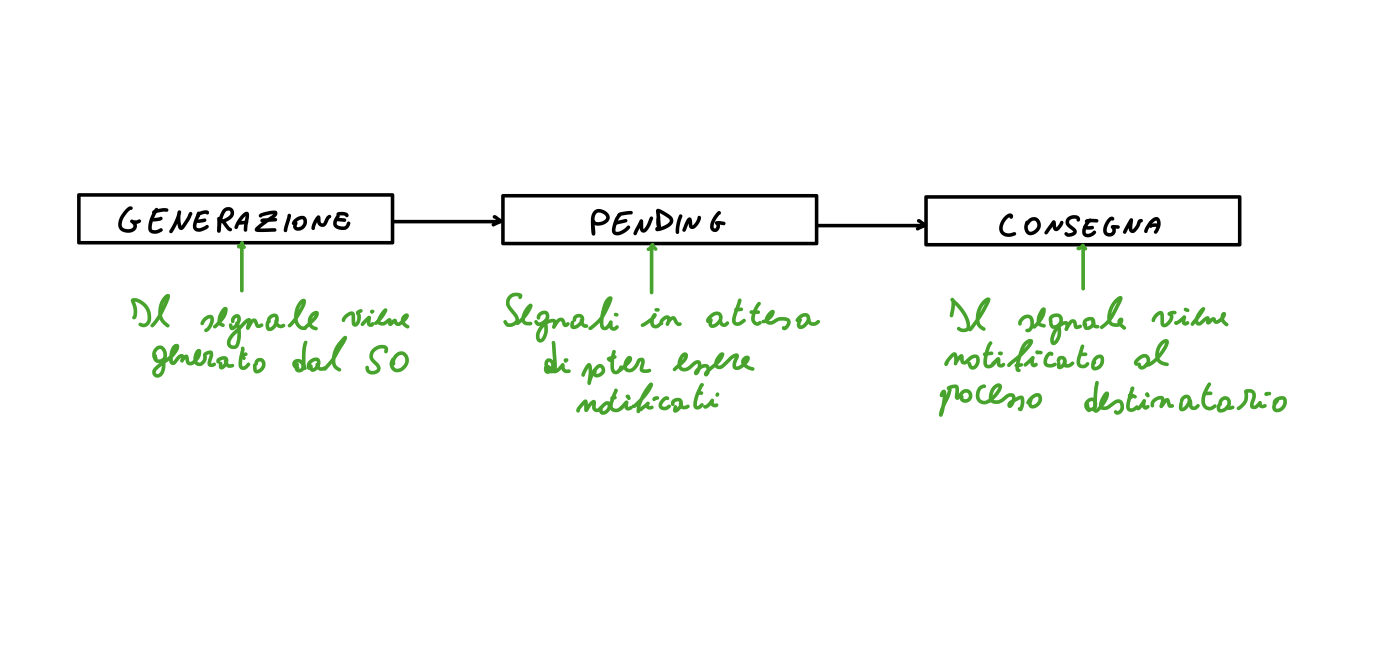
\includegraphics[width=0.9\linewidth]{../images/Ciclo Segnali.png}
    \caption{Ciclo di vita di un segnale}
\end{figure}

\noindent
Il passaggio dallo stato \texttt{Pending} alla consegna del segnale avviene tipicamente:

\begin{itemize}
    \item al ritorno da una \textit{system call};
    \item al termine della gestione di un interrupt.
\end{itemize}

\medskip

\noindent Quando il kernel notifica un segnale a un processo, quest'ultimo può reagire in tre modi differenti:

\begin{enumerate}
    \item \textbf{Term/Core} $\rightarrow$ il processo viene terminato oppure viene generato un \textit{core dump}, cioè una copia dello stato della memoria e della CPU salvata su disco.  
    Il \textit{core dump} è utile per attività di debug e analisi post-mortem.

    \item \textbf{Ignora} $\rightarrow$ il processo ignora il segnale e continua normalmente la propria esecuzione.

    \item \textbf{Catch} $\rightarrow$ il processo intercetta il segnale ed esegue una specifica routine di gestione (\textit{signal handler}).  
    È possibile definire un handler diverso per ciascun segnale oppure utilizzare lo stesso handler per più segnali.  
    Se non viene definito alcun handler personalizzato, viene utilizzata l'azione di default prevista dal sistema.
\end{enumerate}

\begin{figure}[H]
    \centering
    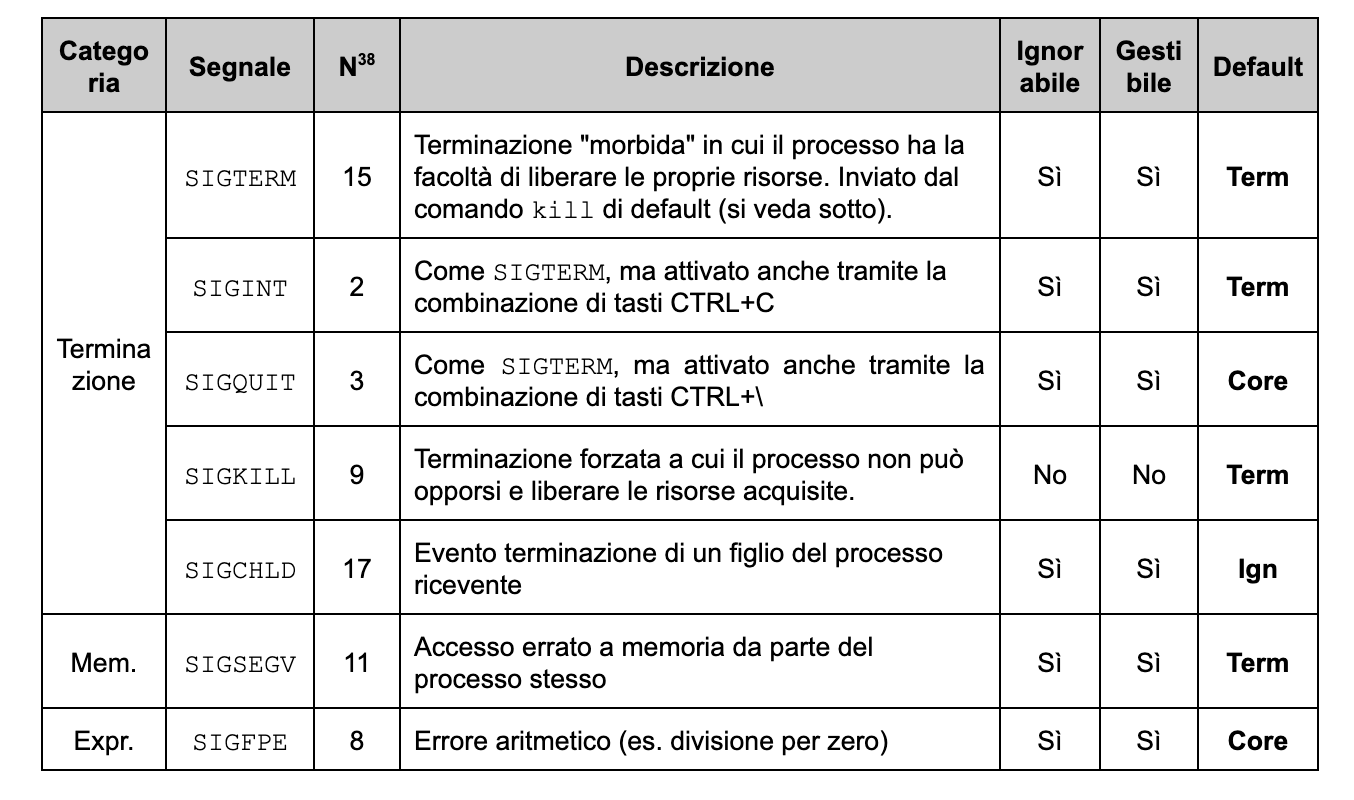
\includegraphics[width=0.9\linewidth]{../images/Tipi di Segnale.png}
    \caption{Principali segnali Linux}
\end{figure}

\noindent
\textbf{\textcolor{red}{Attenzione:}}  
per ogni coppia \textit{processo-segnale} può esistere al massimo un solo segnale nello stato di \texttt{Pending}.  
Se lo stesso segnale viene generato più volte prima della consegna, le notifiche aggiuntive vengono perse.

\medskip

\noindent Spesso la generazione di un interrupt comporta successivamente l'invio di un segnale al processo interessato. Ad esempio:

\begin{verbatim}
UTENTE PREME:

CTRL-C -> interrupt tastiera
        -> interrupt handler
        -> invio SIGINT al processo attivo
        -> gestione del processo

CTRL-Z -> interrupt tastiera
        -> interrupt handler
        -> invio SIGTSTP al processo attivo
        -> gestione del processo

Timer scaduto
        -> interrupt timer
        -> interrupt handler
        -> invio SIGALRM al processo interessato
        -> gestione del processo
\end{verbatim}
\subsection{Gestione dei segnali}
In linguaggio C esistono diverse funzioni per inviare e gestire i segnali.  
Una delle principali funzioni utilizzate per inviare un segnale a un processo è \texttt{kill()}:
\begin{verbatim}
#include <signal.h>
int kill(pid_t pid,   // PID del processo destinatario
         int sig);    // ID del segnale da inviare
\end{verbatim}

\noindent
La funzione invia il segnale identificato da \texttt{sig} al processo avente PID uguale a \texttt{pid}.
\medskip\\
\noindent Un processo può inviare segnali soltanto:
\begin{itemize}
    \item ai propri processi figli;
    \item ai processi appartenenti allo stesso utente;
    \item oppure, nel caso del superutente (\texttt{root}), a qualsiasi processo.
\end{itemize}

\noindent
L'invio di segnali può essere effettuato anche direttamente da terminale tramite il comando:

\begin{verbatim}
kill -9 12345
\end{verbatim}

\noindent
dove:
\begin{itemize}
    \item \texttt{12345} rappresenta il PID del processo destinatario;
    \item \texttt{-9} indica il segnale \texttt{SIGKILL}.
\end{itemize}

\noindent
In generale, il numero associato al comando \texttt{kill} identifica il tipo di segnale da inviare.

\bigskip

\noindent Per gestire un segnale, invece, si utilizza tipicamente la funzione \texttt{sigaction()}:

\begin{verbatim}
#include <signal.h>

int sigaction(int sign,                    // ID del segnale da gestire
              const struct sigaction *act, // Nuova configurazione (indica come gestire il segnale)
              struct sigaction *oldact);   // Vecchia configurazione (se diverso da NULL, 
                                              permette di salvarla)

La funzione restituisce 0 in caso di successo, altrimenti restituisce -1 e imposta errno.
\end{verbatim}

\noindent
I parametri della funzione hanno il seguente significato:

\begin{itemize}
    \item \texttt{sign} $\rightarrow$ identificativo del segnale da configurare;
    
    \item \texttt{act} $\rightarrow$ struttura contenente la nuova modalità di gestione del segnale;
    
    \item \texttt{oldact} $\rightarrow$ se diverso da \texttt{NULL}, permette di salvare la precedente configurazione del segnale.
\end{itemize}

\medskip

\noindent La struttura \texttt{sigaction} è definita nel seguente modo:

\begin{verbatim}
struct sigaction {
    void (*sa_handler)(int);
    void (*sa_sigaction)(int, siginfo_t *, void *);
    sigset_t sa_mask;
    int sa_flags;
    void (*sa_restorer)(void);
};
\end{verbatim}

\noindent
I principali campi della struttura sono:

\begin{itemize}
    \item \texttt{sa\_handler} $\rightarrow$ definisce il comportamento associato al segnale:
    \begin{itemize}
        \item puntatore a una funzione \textit{signal handler};
        \item \texttt{SIG\_IGN} per ignorare il segnale;
        \item \texttt{SIG\_DFL} per utilizzare l'azione di default del sistema.
    \end{itemize}

    \item \texttt{sa\_sigaction} $\rightarrow$ versione avanzata dell'handler che permette di ottenere informazioni aggiuntive sul segnale ricevuto.

    \item \texttt{sa\_mask} $\rightarrow$ insieme di segnali temporaneamente bloccati durante l'esecuzione del signal handler.

    \item \texttt{sa\_flags} $\rightarrow$ insieme di flag che modificano il comportamento dell'handler.  
    Ad esempio, il flag \texttt{SA\_RESTART} permette di riavviare automaticamente alcune system call interrotte da un segnale.

    \item \texttt{sa\_restorer} $\rightarrow$ campo riservato all'uso interno del kernel e normalmente non utilizzato nei programmi applicativi (non utilizzato).
\end{itemize}
\newpage
\section{Gestione della memoria}
Ogni processo vede e utilizza la memoria come se disponesse di uno spazio di indirizzamento lineare e dedicato esclusivamente a sé stesso.  
In realtà, la memoria fisica del sistema è condivisa tra tutti i processi attivi e deve quindi essere gestita dal Sistema Operativo.

\medskip

\noindent Uno dei compiti fondamentali del Sistema Operativo consiste proprio nella gestione della memoria fisica disponibile, garantendo che più processi possano accedervi in modo concorrente, efficiente e sicuro.

\noindent In particolare, il Sistema Operativo deve:

\begin{enumerate}
    \item tenere traccia delle locazioni di memoria fisica attualmente utilizzate;

    \item gestire le nuove richieste di memoria, allocando opportunamente gli spazi liberi disponibili.
\end{enumerate}

\noindent
La gestione della memoria introduce numerosi problemi e aspetti progettuali complessi.  
Per semplicità, ci concentreremo principalmente su questi due aspetti fondamentali.
Immaginiamo che nel Sistema Operativo sia presente un componente software chiamato
\textbf{Allocatore di Memoria} rappresentato da una struttura dati che in ogni istante registra quali
locazioni della memoria fisica sono libere/occupate.\\
I programmi interagiscono con l'allocatore di memoria attraverso, delle primitive di base
che per semplificare possiamo immaginare siano tre:
\begin{enumerate}
    \item p = alloca(n) $\rightarrow$ restituisce l'indirizzo iniziale p di un blocco di memoria 
    contiguo di dimensione pari ad almeno n byte, oppure NULL se non è possibile soddisfare la richiesta.
    In C questa funzione è rappresentata da \texttt{malloc(n)}.
    \item p' = ridimensiona(p, n) $\rightarrow$ ridimensiona il blocco di memoria precedentemente allocato 
    a partire da p purchè abbia una nuova dimensione di almeno n byte.\\
    \textbf{\textcolor{red}{ATTENZIONE:}} il nuovo blocco allocato potrebbe essere raggiungibile 
    ad un nuovo indirizzo p'.
    \item dealloca(p) $\rightarrow$ libera lo spazio di memoria che era stato precedentemente allocato. In 
    C questa funzione è rappresentata da \texttt{free(p)};
\end{enumerate}
\subsection{Frammentazione della memoria}

La \textbf{frammentazione della memoria} è il fenomeno per cui la memoria disponibile risulta suddivisa in più blocchi sparsi e non contigui.  
Di conseguenza, può accadere che una richiesta di allocazione non venga soddisfatta anche se la quantità totale di memoria libera sarebbe sufficiente.

\medskip
\noindent In altre parole, nessuno spazio libero contiguo è abbastanza grande da contenere la nuova allocazione richiesta.
\noindent
Esistono due principali tipi di frammentazione:

\begin{itemize}
    \item \textbf{Frammentazione interna} $\rightarrow$ si verifica quando all'interno di un blocco di memoria allocato rimangono porzioni inutilizzate.  
    Questo accade tipicamente quando l'allocazione avviene in blocchi di dimensione fissa.

    \item \textbf{Frammentazione esterna} $\rightarrow$ si verifica quando una richiesta di allocazione di dimensione \(n\) fallisce perché tutti i blocchi liberi disponibili hanno dimensione inferiore a \(n\), anche se la somma totale della memoria libera sarebbe sufficiente.
\end{itemize}

\medskip

\noindent
\textbf{\textcolor{red}{Attenzione:}}  
la frammentazione esterna può verificarsi soltanto se l'allocatore utilizza blocchi di dimensione variabile.

\begin{figure}[H]
    \centering
    %\includegraphics[width=0.9\linewidth]{../images}
    \caption{Esempio di frammentazione esterna}
\end{figure}

\medskip

\noindent L'allocazione della memoria è tipicamente organizzata su due livelli:

\begin{enumerate}
    \item un primo allocatore, operante in \textit{kernel space}, che gestisce la memoria fisica del sistema e la rende disponibile ai processi;

    \item un secondo allocatore, operante in \textit{user space}, che gestisce la memoria del singolo processo e risponde alle richieste di allocazione dinamica (ad esempio tramite \texttt{malloc()}).
\end{enumerate}
\subsection{Memoria virtuale}
La \textbf{memoria virtuale} è un'astrazione fornita dal Sistema Operativo che consente a ogni processo di utilizzare uno spazio di memoria logico dedicato, indipendente dalla reale disposizione della memoria fisica.

\medskip

\noindent Ogni processo opera utilizzando \textbf{indirizzi logici} (o \textbf{virtuali}), come se avesse a disposizione un'intera memoria privata e continua.  
La traduzione tra indirizzi logici e indirizzi fisici viene effettuata automaticamente dal sistema tramite appositi meccanismi hardware e software.
\begin{center}
\[
\text{Indirizzo logico} \;\longleftrightarrow\; \text{Indirizzo fisico}
\]
\end{center}

\noindent
Dal punto di vista del processo, l'utilizzo della memoria avviene in modo trasparente: il programma non deve preoccuparsi della reale posizione dei dati nella RAM.

\begin{figure}[H]
    \centering
    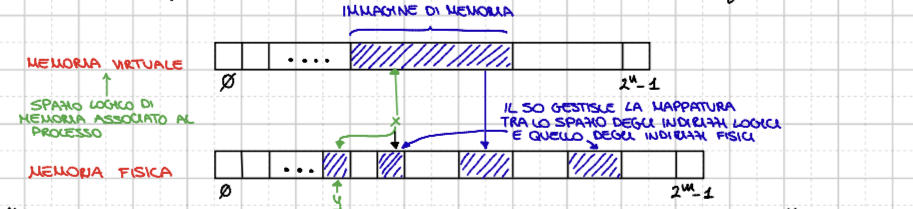
\includegraphics[width=0.9\linewidth]{../images/Gestione Memoria.png}
    \caption{Traduzione tra memoria virtuale e memoria fisica}
\end{figure}

\medskip

\noindent In sintesi, il meccanismo della memoria virtuale permette ai processi di accedere alla memoria fisica attraverso una traduzione automatica degli indirizzi virtuali in indirizzi fisici.

\medskip

\noindent Questo approccio offre numerosi vantaggi:

\begin{itemize}
    \item isolamento tra i processi;
    \item maggiore sicurezza;
    \item utilizzo più efficiente della memoria fisica;
    \item possibilità di eseguire processi più grandi della RAM disponibile;
    \item semplificazione della gestione della memoria da parte dei programmi.
\end{itemize}

\begin{figure}[H]
    \centering
    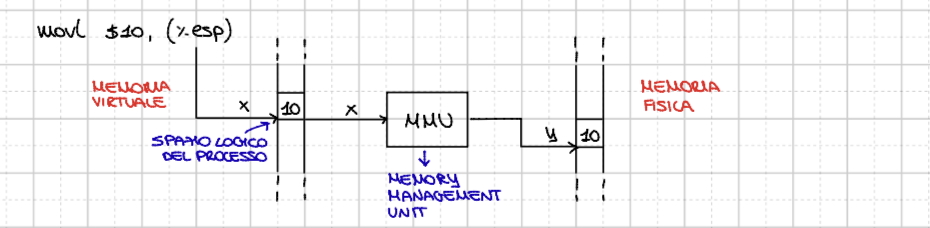
\includegraphics[width=0.9\linewidth]{../images/Allocazione Memoria YEA.png}
    \caption{Vista logica della memoria di un processo}
\end{figure}
\subsection{Paginazione della memoria}
La \textbf{paginazione} è una tecnica di gestione della memoria utilizzata nei moderni sistemi operativi per implementare la memoria virtuale.

\medskip

\noindent Con la paginazione, sia lo spazio di indirizzamento logico sia la memoria fisica vengono suddivisi in blocchi di dimensione fissa:

\begin{itemize}
    \item \textbf{Pagine} (\textit{pages}) $\rightarrow$ blocchi della memoria virtuale;
    
    \item \textbf{Frame} (\textit{page frames}) $\rightarrow$ blocchi della memoria fisica.
\end{itemize}

\noindent
Ogni pagina della memoria virtuale può essere caricata in un qualsiasi frame libero della memoria fisica.

\begin{figure}[H]
    \centering
    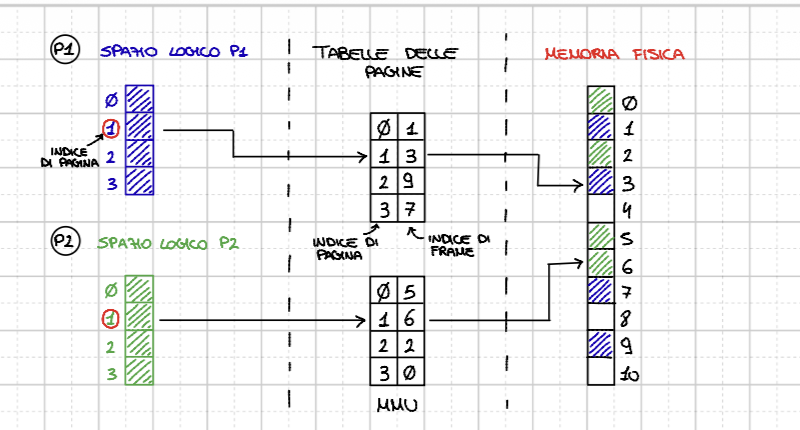
\includegraphics[width=0.9\linewidth]{../images/Paginazione Memoria.png}
    \caption{Paginazione della memoria}
\end{figure}

\medskip

\noindent La traduzione degli indirizzi virtuali in indirizzi fisici viene effettuata dalla \textbf{MMU} (\textit{Memory Management Unit}).

\bigskip

\noindent Supponiamo di avere:

\begin{itemize}
    \item una memoria virtuale di dimensione \(2^v\) byte  
    (ad esempio \(v = 32 \Rightarrow 4\,GB\));

    \item una memoria fisica di dimensione \(2^r\) byte  
    (ad esempio \(r = 33 \Rightarrow 8\,GB\));

    \item pagine di dimensione \(2^d\) byte  
    (ad esempio \(d = 12 \Rightarrow 4\,KB\)).
\end{itemize}

\medskip

\noindent Un indirizzo virtuale di \(v\) bit viene suddiviso in due parti:

\begin{itemize}
    \item \textbf{Numero di pagina} $\rightarrow$ identifica la pagina virtuale;
    
    \item \textbf{Offset} $\rightarrow$ identifica la posizione del dato all'interno della pagina.
\end{itemize}

\noindent
Anche l'indirizzo fisico è composto da:

\begin{itemize}
    \item \textbf{Numero di frame} $\rightarrow$ identifica il frame fisico;
    
    \item \textbf{Offset} $\rightarrow$ stessa posizione relativa all'interno del frame.
\end{itemize}

\begin{figure}[H]
    \centering
    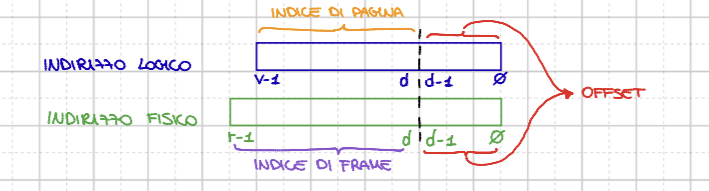
\includegraphics[width=0.9\linewidth]{../images/MMU.png}
    \caption{Traduzione degli indirizzi tramite MMU}
\end{figure}

\medskip

\noindent La traduzione avviene nel seguente modo:

\begin{enumerate}
    \item si estrae dall'indirizzo virtuale il numero di pagina;
    
    \item tramite la \textbf{tabella delle pagine} si individua il frame fisico corrispondente;
    
    \item si concatena il numero di frame con lo stesso offset presente nell'indirizzo virtuale.
\end{enumerate}

\noindent
L'offset rimane invariato perché pagina e frame hanno la stessa dimensione.

\begin{figure}[H]
    \centering
    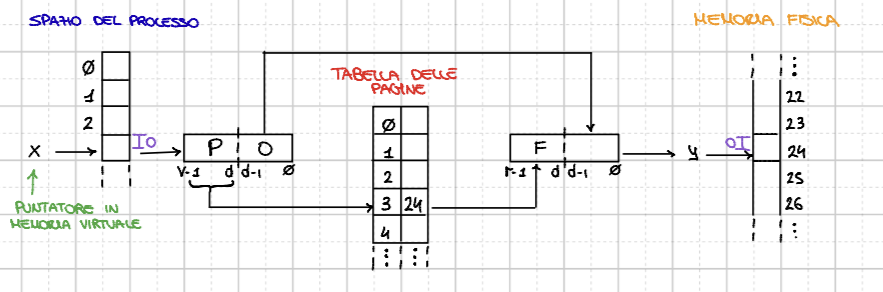
\includegraphics[width=0.9\linewidth]{../images/Traduzione.png}
    \caption{Schema di traduzione da indirizzo virtuale a indirizzo fisico}
\end{figure}
\subsection{Paginazione con bit di validità}
Ad ogni riga della tabela delle pagine aggiungo un bit di validità con seguente significato:
\begin{itemize}
    \item 0 pagina inutilizzata (non valida)
    \item 1 pagina in uso (valida)
\end{itemize}
\begin{figure}[H]
    \centering  
    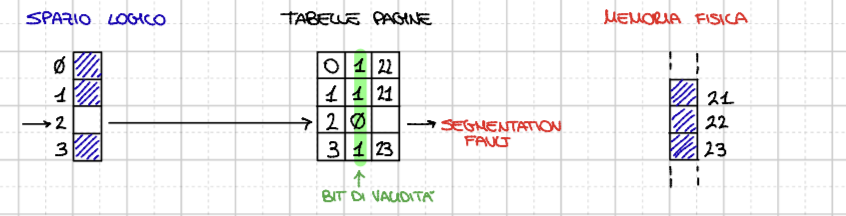
\includegraphics[width=0.9\linewidth]{../images/Paginazione validita.png}
    \caption{Paginazione bit validità}
    %\label{label}
\end{figure}
\subsection{Memory swapping}
Il \textbf{memory swapping} è una tecnica utilizzata dal Sistema Operativo per gestire situazioni in cui la memoria fisica non è sufficiente a contenere tutte le pagine attive dei processi.

\medskip

\noindent Spesso accade che alcune pagine di memoria, pur essendo valide, rimangano inutilizzate per lunghi periodi di tempo.  
Quando la memoria fisica è satura, il sistema può trasferire alcune di queste pagine su disco per liberare spazio: questa operazione prende il nome di \textbf{swap-out}.

\medskip

\noindent Quando un processo tenta di accedere a una pagina che è stata precedentemente spostata su disco, si verifica un \textbf{page fault}.  
In questo caso, il Sistema Operativo deve recuperare la pagina dalla memoria secondaria e riportarla in RAM tramite un’operazione di \textbf{swap-in}, permettendo al processo di proseguire l’esecuzione.

\bigskip

\noindent
Il funzionamento può essere riassunto nei seguenti passi:

\begin{enumerate}
    \item la CPU genera un interrupt di tipo \textit{page fault};
    
    \item il kernel seleziona un frame “vittima” nella memoria fisica;
    
    \item il contenuto del frame vittima viene salvato su disco (\textit{swap-out});
    
    \item la pagina richiesta viene caricata nel frame liberato (\textit{swap-in});
    
    \item le tabelle delle pagine vengono aggiornate per riflettere la nuova mappatura;
    
    \item il processo viene riattivato e ripete l’istruzione che aveva causato il page fault.
\end{enumerate}

\medskip

\noindent Questo meccanismo viene spesso indicato come \textbf{paginazione con swap e bit di validità}.

\bigskip

\noindent
I principali vantaggi e svantaggi sono:

\begin{verbatim}
VANTAGGI:
+ Tutti i processi condividono uno spazio di indirizzamento virtuale
+ Migliore utilizzo della memoria fisica (solo le pagine attive restano in RAM)
+ Possibilità di utilizzare più memoria di quella fisicamente disponibile

SVANTAGGI:
- Fenomeno di thrashing (continui swap che degradano le prestazioni)
- Maggiore complessità nella gestione della memoria
- Dipendenza dalla presenza di memoria secondaria veloce (disco/SSD)
\end{verbatim}
\subsection{Allocazione della memoria}
Quando viene invocata la funzione \texttt{malloc(x)}, la memoria richiesta viene allocata all’interno dell’\textbf{heap} del processo.
\begin{figure}[H]
    \centering
    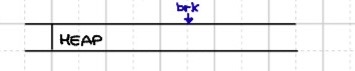
\includegraphics[width=0.5\linewidth]{../images/Allocazione Memoria YEA YEa.jpg}
    \caption{Struttura dell'heap}
\end{figure}

\medskip

\noindent Il puntatore \textbf{brk} definisce il limite superiore dell’heap, ovvero la massima area attualmente allocata.  
Questo limite può essere modificato tramite la system call \texttt{sbrk()}.

\bigskip

\noindent La gestione dell’heap suddivide lo spazio disponibile in tre tipologie di aree:

\begin{enumerate}
    \item memoria allocata e attualmente utilizzata dal processo;
    \item memoria libera, disponibile per nuove allocazioni;
    \item memoria occupata da strutture di gestione (metadati).
\end{enumerate}

\medskip

\noindent Lo spazio dell’heap è organizzato in \textbf{blocchi}, ciascuno dei quali può appartenere a una delle categorie precedenti.  
I blocchi sono disgiunti tra loro e contengono sempre un’intestazione (\textit{header}) con informazioni di gestione.

\begin{figure}[H]
    \centering
    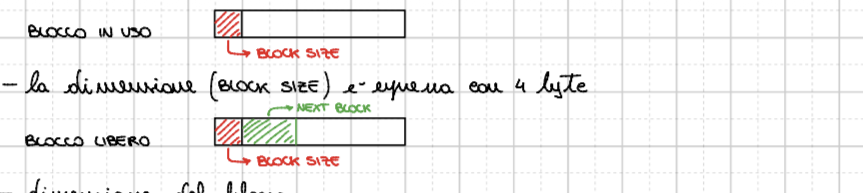
\includegraphics[width=0.9\linewidth]{../images/bllocchi.png}
    \caption{Struttura dei blocchi di memoria}
\end{figure}

\bigskip

\noindent I blocchi liberi sono organizzati in una struttura dati chiamata \texttt{free\_list}, tipicamente implementata come lista concatenata.

\begin{verbatim}
p = malloc(n)
-> cerca nella free_list un blocco libero di dimensione S >= n + overhead
-> dimensione minima tipica di un blocco: 12 byte
\end{verbatim}

\noindent
Se viene trovato un blocco adatto, questo viene rimosso dalla \texttt{free\_list}.  
La scelta del blocco può seguire diverse strategie:

\begin{itemize}
    \item \textbf{First-Fit} $\rightarrow$ seleziona il primo blocco sufficientemente grande;
    
    \item \textbf{Best-Fit} $\rightarrow$ seleziona il blocco più piccolo tra quelli disponibili che soddisfano la richiesta, riducendo la frammentazione interna.
\end{itemize}

\medskip

\noindent Se non è disponibile alcun blocco adeguato, l’heap viene esteso aumentando il valore di \texttt{brk} e creando un nuovo blocco di dimensione adeguata.

\begin{verbatim}
free(p)
-> inserisce il blocco puntato da (p - header) nella free_list
\end{verbatim}
\subsection{Altri miglioramenti}
\begin{itemize}
    \item Fusione di blocchi liberi adiaceni 
    \begin{figure}[H]
    \centering  
    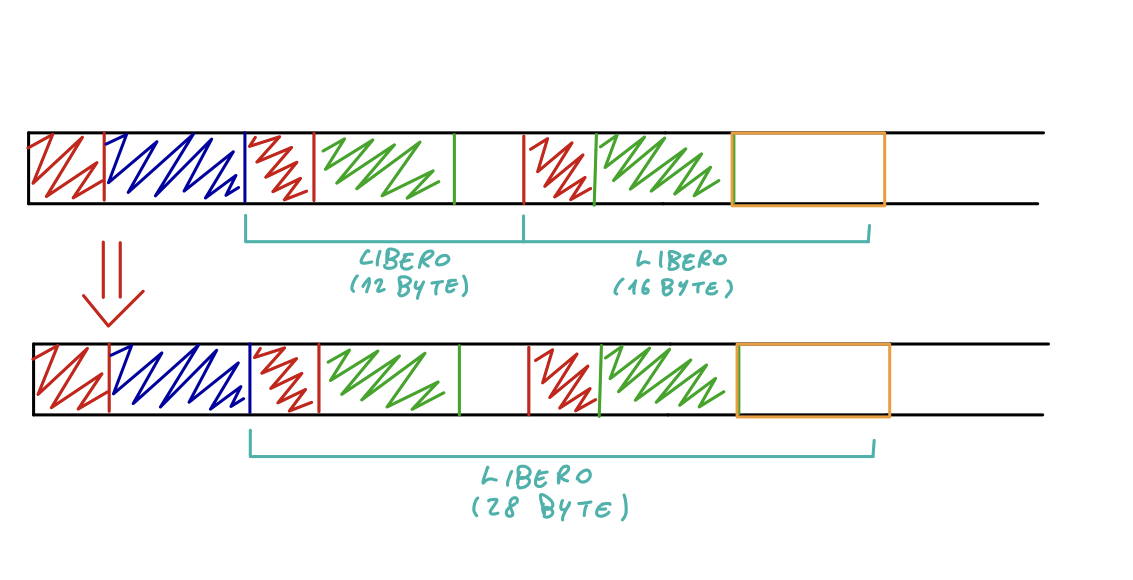
\includegraphics[width=0.9\linewidth]{../images/Fusione a blocchi.png}
    \caption{Fusioni di blocchi liberi adiacenti}
    %\label{label}
    \end{figure}
    \item Partizionamento dei blocchi liberi
    \begin{figure}[H]
    \centering  
    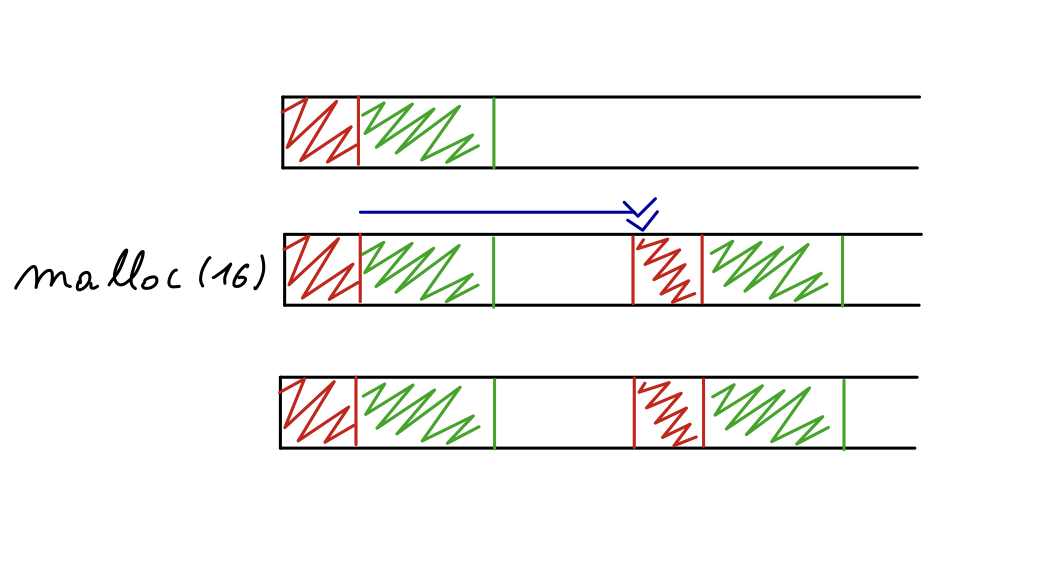
\includegraphics[width=0.5\linewidth]{../images/Partizione a bocchi.png}
    \caption{Partizionamento dei blocchi liberi}
    %\label{label}
    \end{figure}
    \item Liste free separate per blochi di dimensioni diverse
    \item Allineamento 
\end{itemize}
\subsection{Cache e uso ottimizzato della memoria}
Consideriamo due operazioni a livello di assembly:
\begin{verbatim}
movl $1, %eax     -> 1 ns
movl $1, (%eax)   -> 100 ns
\end{verbatim}

\noindent
Si nota come l’accesso alla memoria sia significativamente più lento rispetto alle operazioni sui registri.

\medskip

\noindent La \textbf{cache} è una memoria ad alta velocità che conserva temporaneamente i dati utilizzati più frequentemente, riducendo il tempo medio di accesso alla memoria principale.

\noindent Essa è organizzata in \textbf{linee (cache lines)} di dimensione fissa (ad esempio 64 byte).  
Ogni linea contiene una copia di una porzione della memoria principale.

\bigskip

\noindent Ogni indirizzo di memoria \(X\) è associato a un blocco di cache identificato come:

\[
\left\lfloor \frac{X}{L} \right\rfloor
\]

\noindent dove \(L\) rappresenta la dimensione della cache line.

\medskip

\noindent Quando si accede a un indirizzo di memoria, possono verificarsi due casi:

\begin{itemize}
    \item \textbf{Cache hit} $\rightarrow$ il dato è già presente in cache e può essere letto rapidamente;

    \item \textbf{Cache miss} $\rightarrow$ il dato non è presente in cache e deve essere caricato dalla memoria principale.
\end{itemize}

\medskip

\noindent Se la cache è piena, è necessario sostituire una linea esistente secondo una politica di rimpiazzo.

\noindent La progettazione della cache si basa sui principi di località:

\begin{itemize}
    \item \textbf{Località temporale} $\rightarrow$ se un dato viene acceduto, è probabile che venga riutilizzato nel breve periodo;

    \item \textbf{Località spaziale} $\rightarrow$ se un indirizzo viene acceduto, è probabile che vengano acceduti anche indirizzi vicini.
\end{itemize}

\bigskip

\noindent
\textbf{Esempio:}

\begin{verbatim}
int sum(int **m, int n){
    int i, j, s = 0;

    for(i = 0; i < n; i++)
        for(j = 0; j < n; j++)
            s = s + m[i][j];

    return s;
}
\end{verbatim}

\noindent
Questa versione sfrutta la località spaziale (accesso per righe) ed è quindi più efficiente.

\medskip

\noindent Se invece si accede agli elementi in ordine trasposto:

\begin{verbatim}
m[j][i]
\end{verbatim}

\noindent
si perde la località spaziale, causando molti più cache miss e un aumento significativo del tempo di esecuzione (ad esempio da 0.3s a 1.5s).
\newpage
\section{Cache e associatività}
La \textbf{cache} è una memoria ad accesso rapido organizzata in blocchi di dimensione fissa, chiamati \textbf{linee di cache} (\textit{cache lines}).
Ogni linea contiene una copia di una porzione della memoria principale, permettendo di ridurre significativamente i tempi di accesso ai dati più utilizzati.
\medskip

\noindent La cache non è gestita direttamente dai programmi applicativi, ma dal sistema hardware e dal Sistema Operativo.

\noindent Ogni linea di cache è associata a un \textbf{tag}, utilizzato per identificare quale blocco di memoria principale è attualmente memorizzato nella linea.

\begin{figure}[H]
    \centering
    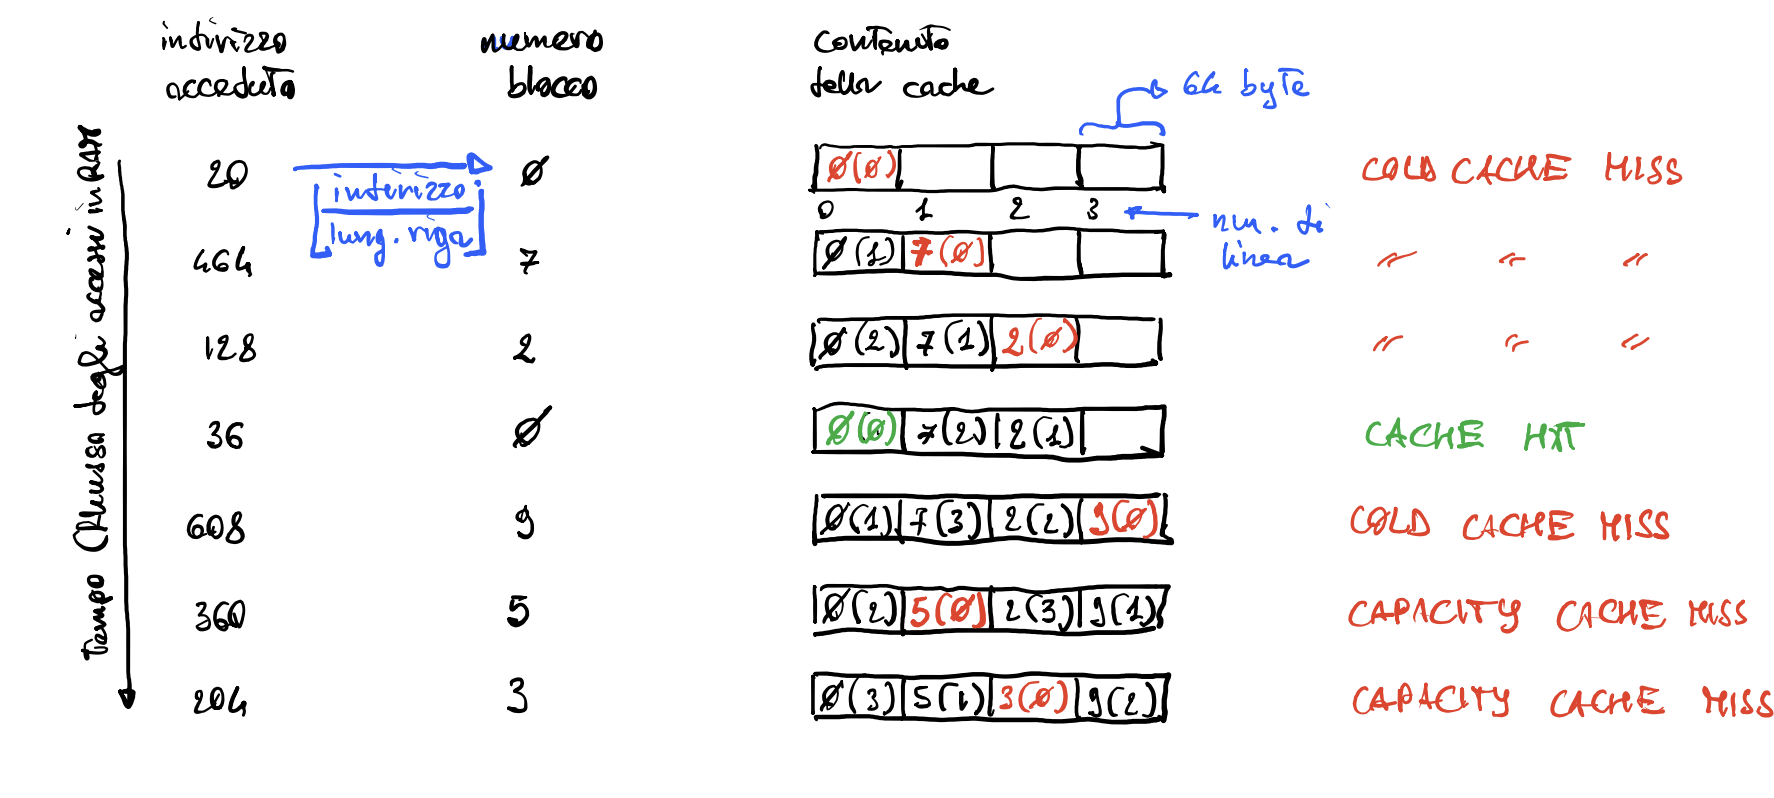
\includegraphics[width=0.9\linewidth]{../images/Cache esempio .png}
    \caption{Esempio di organizzazione della cache}
\end{figure}

\bigskip

\subsection*{Tipologie di cache}

\noindent Esistono tre principali modalità di organizzazione della cache.

\begin{itemize}

    \item \textbf{Cache completamente associativa} (\textit{fully associative}) $\rightarrow$
    ogni blocco di memoria può essere memorizzato in qualsiasi linea della cache.

\begin{verbatim}
VANTAGGI
+ utilizzo molto efficiente dello spazio in cache
+ riduzione dei conflict miss

SVANTAGGI
- implementazione complessa
- costo hardware elevato
\end{verbatim}

\bigskip

    \item \textbf{Cache associativa a k-vie} (\textit{k-way set associative}) $\rightarrow$
    ogni blocco di memoria può essere memorizzato solo in un insieme (\textit{set}) specifico di \(k\) linee, determinato tramite una funzione di mapping.

\medskip

    Questo approccio rappresenta un compromesso tra:
    \begin{itemize}
        \item efficienza della cache completamente associativa;
        \item semplicità della cache a mappatura diretta.
    \end{itemize}

\bigskip

    \item \textbf{Cache a mappatura diretta} (\textit{direct mapped}) $\rightarrow$
    ogni blocco di memoria può essere memorizzato in una sola linea specifica della cache.

\begin{verbatim}
VANTAGGI
+ implementazione semplice
+ costo ridotto
+ accesso molto veloce

SVANTAGGI
- maggiore probabilità di cache miss
- utilizzo meno efficiente della cache
\end{verbatim}

\end{itemize}

\begin{figure}[H]
    \centering
    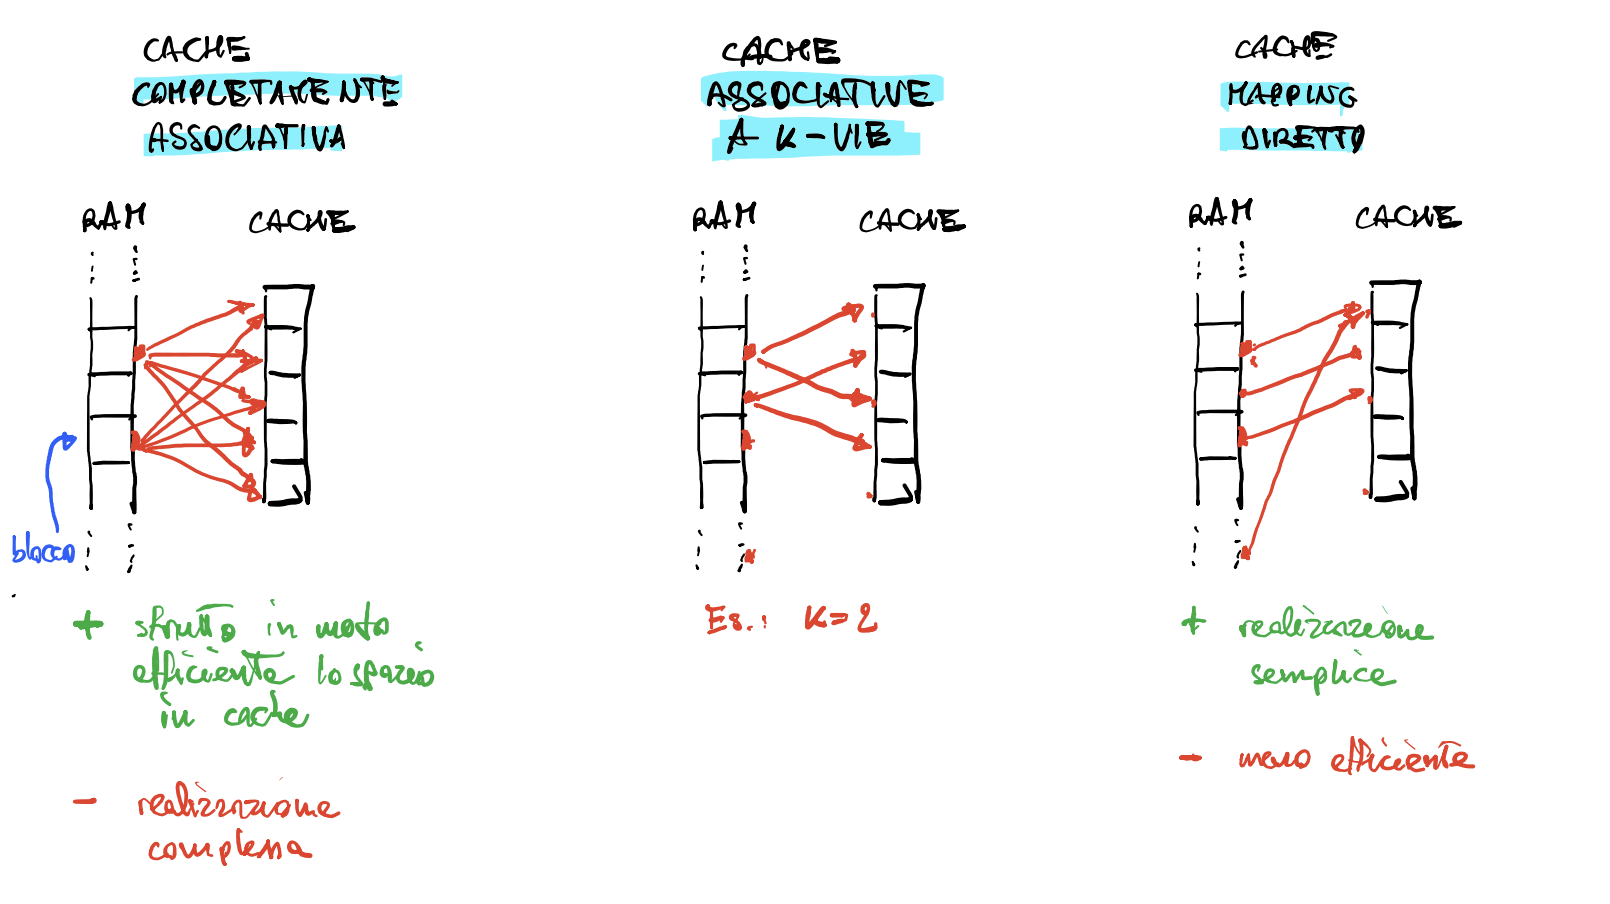
\includegraphics[width=0.9\linewidth]{../images/tipi cache.png}
    \caption{Confronto tra i diversi tipi di cache}
\end{figure}

\bigskip

\subsection*{Tipologie di cache miss}

A seconda dell’organizzazione della cache e dello stato corrente della memoria,
durante un accesso possono verificarsi differenti situazioni.

\begin{itemize}

    \item \textbf{Cache hit} $\rightarrow$
    il dato richiesto è già presente nella cache e può essere letto rapidamente.

\medskip

    \item \textbf{Cache miss} $\rightarrow$
    il dato richiesto non è presente nella cache e deve essere caricato dalla memoria principale.

\medskip

    \item \textbf{Capacity miss} $\rightarrow$
    la cache è piena e il caricamento del nuovo dato richiede la sostituzione di una linea esistente (linea vittima).

\medskip

    \item \textbf{Conflict miss} $\rightarrow$
    il dato non può essere inserito perché la linea di cache assegnata è già occupata da un altro blocco incompatibile.

\medskip

\noindent Questo fenomeno si verifica principalmente nelle cache a mappatura diretta o nelle cache associative con pochi modi.
\end{itemize}

\newpage
\section{File System}
Il \textbf{File System} è l’insieme delle strutture organizzative e delle funzionalità attraverso cui il Sistema Operativo gestisce i dati memorizzati nei dispositivi di archiviazione.
In altre parole, rappresenta il livello software che consente al Sistema Operativo di interfacciarsi con le periferiche di memoria (dischi, SSD, chiavette USB, ecc.) organizzando i dati in modo strutturato ed efficiente.

\begin{figure}[H]
    \centering
    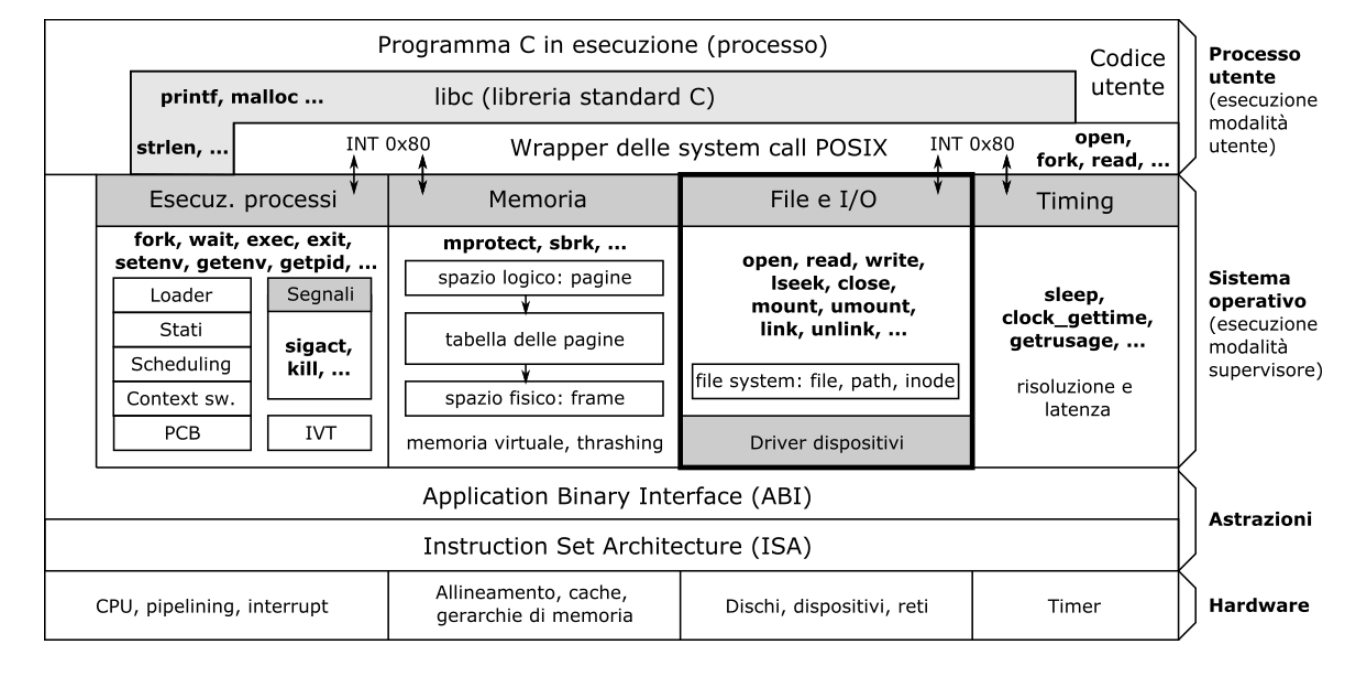
\includegraphics[width=0.9\linewidth]{../images/File Systemm.png}
    \caption{Architettura generale del File System}
\end{figure}

\bigskip

\noindent
Analizziamo ora i principali elementi che compongono un file system.

\subsection{File e Directory}
\subsubsection*{File}

Un \textbf{file} è un contenitore di dati, generalmente rappresentati come una sequenza ordinata di byte.
Oltre al contenuto vero e proprio, ogni file possiede una serie di \textbf{metadati}, utilizzati dal Sistema Operativo per gestirlo correttamente.

\noindent Tra i principali metadati troviamo:

\begin{itemize}
    \item \textbf{Nome} del file;
    
    \item \textbf{Dimensione} in byte;
    
    \item \textbf{Permessi di accesso};
    
    \item \textbf{Timestamp} (creazione, modifica, ultimo accesso).
\end{itemize}

\begin{figure}[H]
    \centering
    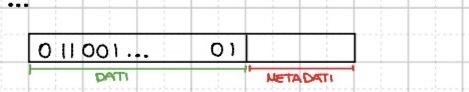
\includegraphics[width=0.9\linewidth]{../images/fileeeee.jpg}
    \caption{Esempio di file con metadati}
\end{figure}

\bigskip

\subsubsection*{Directory}

Una \textbf{directory} è un contenitore logico utilizzato per organizzare file e altre directory.

\noindent Le directory permettono di strutturare i dati secondo una gerarchia, tipicamente ad albero, facilitando la navigazione e la gestione delle informazioni all’interno del file system.

\begin{figure}[H]
    \centering
    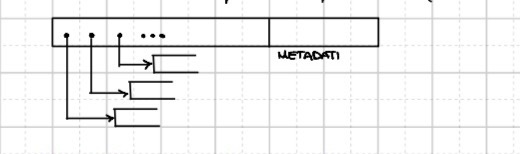
\includegraphics[width=0.9\linewidth]{../images/dirrreeeee.jpg}
    \caption{Organizzazione gerarchica delle directory}
\end{figure}
\subsection{Struttura gerarchica dei File System}
Nei sistemi UNIX/Linux, il contenuto del file system è organizzato secondo una struttura gerarchica ad albero.
Alla base di questa struttura si trova una directory speciale chiamata \textbf{root directory}, identificata dal simbolo:

\[
/
\]

\noindent
Tutti i file e le directory presenti nel sistema discendono da questa directory principale.

\begin{figure}[H]
    \centering
    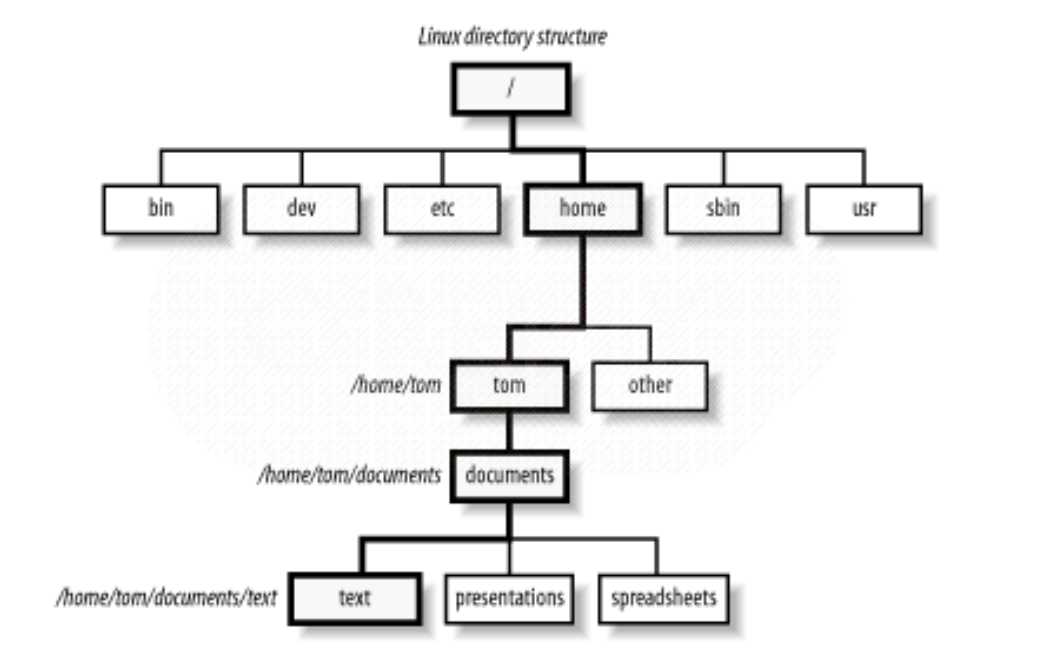
\includegraphics[width=0.9\linewidth]{../images/UNIX DIRECTORY.png}
    \caption{Struttura gerarchica del file system UNIX}
\end{figure}

\bigskip

\noindent
Ogni directory, ad eccezione della root directory, possiede una \textbf{directory genitore}.

\noindent Se una directory è contenuta all’interno di un’altra directory, allora viene detta \textbf{directory figlia}.

\noindent Ad esempio, nella figura:

\begin{itemize}
    \item \texttt{tom} e \texttt{other} sono directory figlie di \texttt{home};
    
    \item \texttt{home} è la directory genitore di \texttt{tom} e \texttt{other}.
\end{itemize}

\medskip

\noindent I file system UNIX-like sono generalmente \textbf{case-sensitive}: lettere maiuscole e minuscole vengono considerate differenti.

\noindent Ad esempio:

\begin{verbatim}
/home/tom/documents/text
\end{verbatim}

\noindent
e

\begin{verbatim}
/home/tom/documents/Text
\end{verbatim}

\noindent
identificano due file distinti.

\bigskip

\noindent
Il \textbf{Filesystem Hierarchy Standard (FHS)} è uno standard che definisce l’organizzazione e il significato delle principali directory nei sistemi UNIX/Linux, garantendo uniformità tra le diverse distribuzioni.

\bigskip
\subsection{Path / Percorso}

Nel file system, ogni file o directory è identificato univocamente tramite un \textbf{path} (percorso).

Esistono due tipologie principali di path:

\begin{itemize}

    \item \textbf{Path assoluto} $\rightarrow$ rappresenta il percorso completo che parte dalla root directory e arriva fino al file o directory desiderato.

\begin{verbatim}
/home/Tom/Documents/Text
\end{verbatim}

\noindent
In questo esempio:

\begin{itemize}
    \item \texttt{Text} è il file/directory identificato;
    
    \item \texttt{home}, \texttt{Tom} e \texttt{Documents} rappresentano le directory attraversate;
    
    \item il simbolo iniziale \texttt{/} identifica la root directory;
    
    \item gli altri caratteri \texttt{/} fungono da separatori.
\end{itemize}

\medskip

\noindent
\textbf{\textcolor{red}{Attenzione:}}
\begin{verbatim}
/      -> path valido
//     -> generalmente non considerato un path standard
\end{verbatim}

\bigskip

    \item \textbf{Path relativo} $\rightarrow$ rappresenta il percorso rispetto a una directory di riferimento (tipicamente la directory corrente).
    
\end{itemize}

\medskip

Per costruire path relativi si utilizzano alcuni riferimenti speciali:

\begin{itemize}
    \item \texttt{.} $\rightarrow$ directory corrente;
    
    \item \texttt{..} $\rightarrow$ directory padre;
    
    \item \texttt{\textasciitilde} $\rightarrow$ home directory dell’utente corrente.
\end{itemize}

\bigskip

\noindent
\textbf{Esempio}

Supponiamo di trovarci nella directory:

\begin{verbatim}
/home/tom/documents
\end{verbatim}

\noindent
Per raggiungere la directory \texttt{other}:

\begin{verbatim}
../../other
\end{verbatim}

\noindent
Il percorso:
\begin{itemize}
    \item torna indietro di due livelli tramite \texttt{..};
    
    \item entra successivamente nella directory \texttt{other}.
\end{itemize}
\subsection{Organizzazione interna del File System}
Per descrivere l’organizzazione interna di un file system consideriamo i file system della famiglia \texttt{ext} (ad esempio \texttt{ext2}, \texttt{ext3}, \texttt{ext4}), tipici dei sistemi UNIX/Linux.
\medskip

\noindent In questi file system, ogni file o directory è associato a una struttura dati chiamata \textbf{inode} (\textit{index node}).

\noindent L’inode contiene tutte le informazioni necessarie alla gestione del file, ad eccezione del nome, ed è caricato e gestito dal Sistema Operativo.

\medskip

\noindent I dati effettivi del file non sono memorizzati direttamente nell’inode, ma in blocchi separati di dimensione fissa presenti sul disco.

\bigskip

\subsubsection*{Contenuto di un inode}
Un inode contiene principalmente metadati relativi al file:

\begin{itemize}
    \item \textbf{Numero inode} $\rightarrow$ identificatore univoco nella tabella degli inode;
    
    \item \textbf{Tipo di oggetto} $\rightarrow$ file regolare, directory, link simbolico, ecc.;
    
    \item \textbf{Permessi di accesso};
    
    \item \textbf{Numero di hard link};
    
    \item \textbf{User ID (UID)} $\rightarrow$ identificativo del proprietario;
    
    \item \textbf{Group ID (GID)} $\rightarrow$ identificativo del gruppo proprietario;
    
    \item \textbf{Dimensione del file};
    
    \item \textbf{Timestamp}:
    \begin{itemize}
        \item ultimo accesso;
        \item ultima modifica del contenuto;
        \item ultima modifica dell’inode;
        \item creazione del file.
    \end{itemize}
\end{itemize}

\medskip

\noindent Queste informazioni permettono al Sistema Operativo di gestire il file e ricostruirne la cronologia delle operazioni effettuate.

\bigskip

\subsubsection*{Permessi di accesso}
I permessi definiscono quali operazioni possono essere effettuate sul file.
Per ciascuna categoria di utenti sono disponibili tre diritti:

\begin{itemize}
    \item \textbf{R} (\textit{Read}) $\rightarrow$ lettura;
    
    \item \textbf{W} (\textit{Write}) $\rightarrow$ scrittura;
    
    \item \textbf{X} (\textit{Execute}) $\rightarrow$ esecuzione.
\end{itemize}

\medskip

\noindent I permessi vengono specificati per:

\begin{enumerate}
    \item utente proprietario;
    \item gruppo proprietario;
    \item tutti gli altri utenti.
\end{enumerate}

\begin{verbatim}
RWX RWX RWX
 |   |   |
 |   |   +--> altri utenti
 |   +------> gruppo
 +----------> proprietario
\end{verbatim}

\medskip

\noindent Esempio:

\begin{verbatim}
r-x r-x r-x
\end{verbatim}

\noindent
significa che:

\begin{itemize}
    \item il proprietario può leggere ed eseguire;
    
    \item il gruppo può leggere ed eseguire;
    
    \item tutti gli altri utenti possono leggere ed eseguire.
\end{itemize}

\bigskip

\noindent Per modificare i permessi si utilizza il comando:

\begin{verbatim}
chmod
\end{verbatim}

\noindent
mentre per modificare proprietario o gruppo si utilizza:

\begin{verbatim}
chown
\end{verbatim}

\medskip

\noindent Esempi:

\begin{verbatim}
chmod a+r text.txt
chmod g-x file.txt
\end{verbatim}

\bigskip

\subsubsection*{Notazione ottale dei permessi}
I permessi possono essere rappresentati anche in forma ottale (base 8):

\begin{center}
\begin{tabular}{c|c}
Permesso & Valore \\ \hline
R & 4 \\
W & 2 \\
X & 1
\end{tabular}
\end{center}

\medskip

\noindent Ad esempio:

\begin{verbatim}
755
\end{verbatim}

\noindent
corrisponde a:

\begin{verbatim}
rwx r-x r-x
\end{verbatim}

\medskip

\noindent Quando un file viene creato da un programma, i permessi iniziali possono essere specificati tramite la system call:

\begin{verbatim}
open()
\end{verbatim}

\bigskip

\subsubsection*{Puntatori ai dati}
L’inode contiene anche i puntatori ai blocchi dati del file.

\noindent Tipicamente sono presenti:

\begin{itemize}
    \item 12 puntatori diretti;
    
    \item 1 puntatore indiretto singolo;
    
    \item 1 puntatore indiretto doppio.
\end{itemize}

\medskip

\noindent I puntatori diretti referenziano direttamente i blocchi contenenti i dati.

\noindent I puntatori indiretti, invece, referenziano blocchi che contengono ulteriori indirizzi di blocchi dati.

\begin{figure}[H]
    \centering
    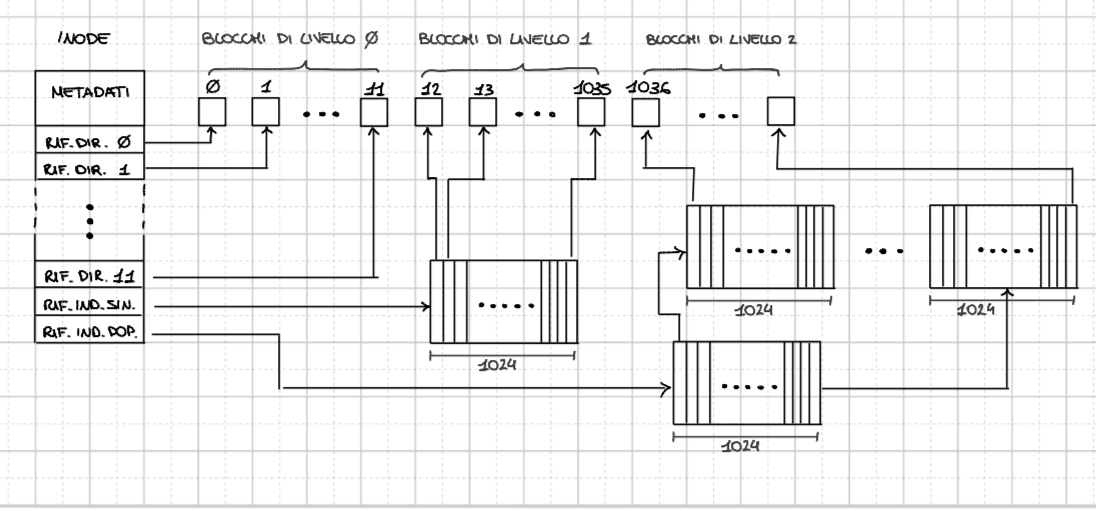
\includegraphics[width=0.9\linewidth]{../images/Inode.png}
    \caption{Schema di un inode}
\end{figure}

\bigskip

\noindent Assumendo blocchi da \(4\,KB\):

\begin{verbatim}
Dimensione massima file =
12 * 4096
+ 1024 * 4096
+ 1024^2 * 4096
= 4 GB
\end{verbatim}

\medskip

\noindent Lo spazio occupato dagli indici è:

\begin{verbatim}
(12 + 2) * 4 + 4096 + (1024 + 1) * 4096
= 4 MB
\end{verbatim}

\bigskip

\subsubsection*{Directory}
Anche le directory sono rappresentate tramite inode.
I dati contenuti in una directory consistono tipicamente in associazioni:

\[
\texttt{nome file} \rightarrow \texttt{numero inode}
\]

\begin{figure}[H]
    \centering
    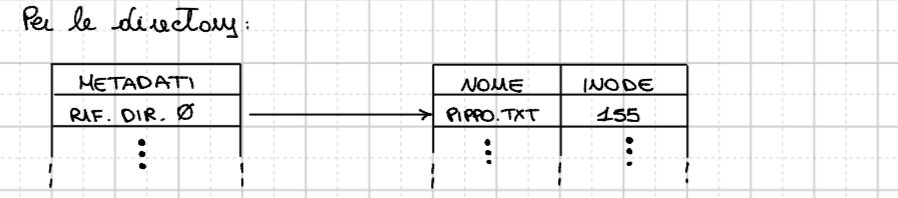
\includegraphics[width=0.9\linewidth]{../images/aiutttt.png}
    \caption{Struttura interna di una directory}
\end{figure}

\bigskip

\subsubsection*{Esempi di occupazione su disco}

\paragraph{File da 265 byte}

\begin{verbatim}
Occupa 1 blocco -> 4 KB
\end{verbatim}

\paragraph{File da 16000 byte}

\begin{verbatim}
16000 / 4096 = 4 blocchi
Occupa quindi 16 KB
\end{verbatim}

\paragraph{File da 4 MB}

\begin{verbatim}
4 MB = 4194304 byte

4194304 / 4096 = 1024 blocchi

12 blocchi -> indirizzati direttamente
1012 blocchi -> tramite indirizzamento indiretto singolo
+ 1 blocco aggiuntivo per contenere i puntatori indiretti

Totale spazio occupato:
(12 + 1012 + 1) * 4096
\end{verbatim}
\subsection{Tabella dei descrittori}
Per ogni processo, il sistema operativo mantiene una \textbf{tabella dei descrittori}
(File Descriptor Table), contenente l’elenco dei file e degli stream di I/O aperti dal processo.

\noindent Ogni voce della tabella associa un \textbf{file descriptor} (intero non negativo)
a una struttura del kernel che rappresenta un file aperto, includendo:
\begin{itemize}
    \item posizione corrente nel file;
    \item modalità di accesso (lettura, scrittura, append, \dots);
    \item riferimento all’inode del file.
\end{itemize}

\begin{figure}[H]
    \centering  
    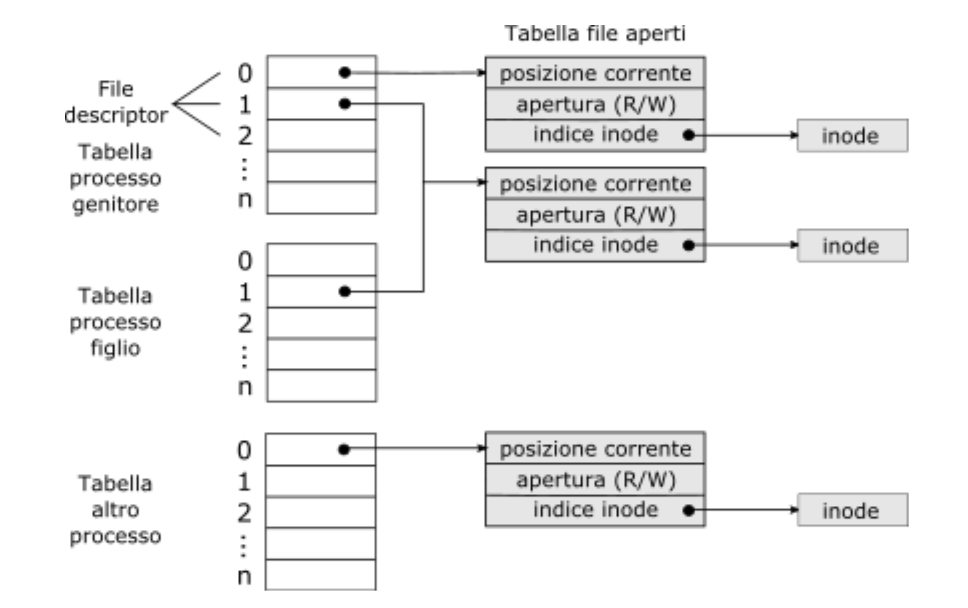
\includegraphics[width=0.6\linewidth]{../images/Tabella Dei Descrittori.png}
    \caption{Tabella dei descrittori dei file aperti}
\end{figure}

\noindent Esempio:
\begin{verbatim}
x = fopen("a.txt");

if (fork() == 0)
    y = fopen("b.txt");
else
    z = fopen("c.txt");
\end{verbatim}

\noindent Dopo la chiamata a \texttt{fork()}, il processo figlio eredita una copia
della tabella dei descrittori del padre. Inizialmente, quindi, padre e figlio
condividono gli stessi file aperti.

\noindent \textbf{\textcolor{red}{ATTENZIONE:}} in presenza di thread multipli,
la tabella dei descrittori è condivisa tra tutti i thread dello stesso processo.

\vspace{0.3cm}

\subsection{Gestione (Mount) dei Dispositivi}
L’operazione di \texttt{mount} rende accessibile il file system di un dispositivo
all’interno della struttura gerarchica unica del file system UNIX.

\noindent In pratica, il contenuto del dispositivo viene associato a una directory detta
\textbf{punto di mount} (\textit{mount point}).

\begin{figure}[H]
    \centering  
    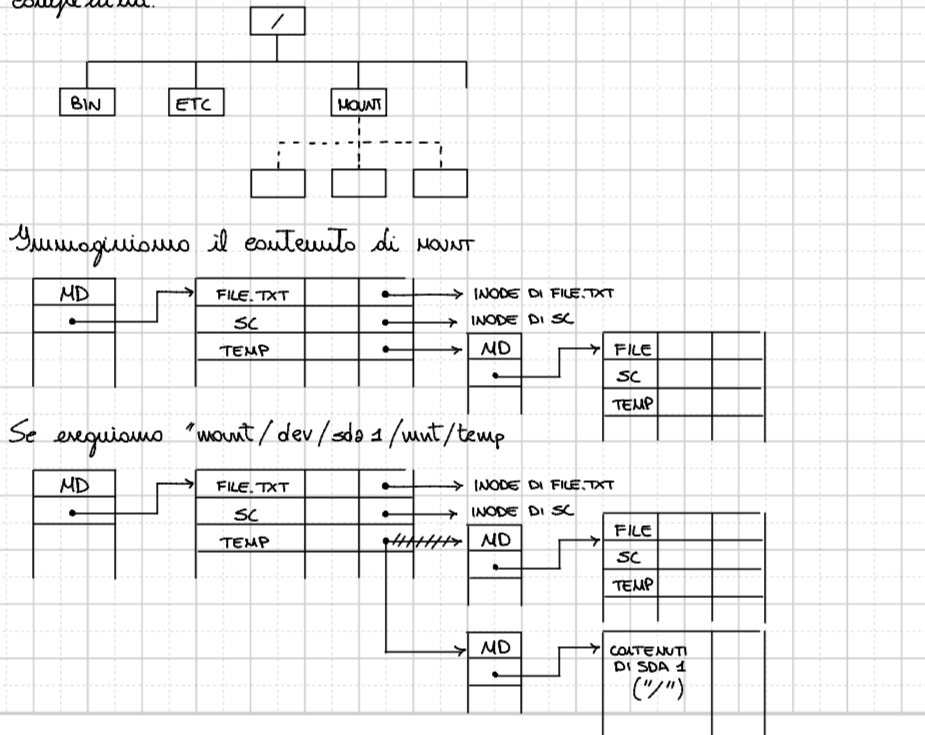
\includegraphics[width=0.6\linewidth]{../images/Mount.png}
    \caption{Operazione di mount}
\end{figure}
\newpage
\noindent Esempio:
\begin{verbatim}
/dev/sdb1 --> montato su --> /mnt/usb
\end{verbatim}

\noindent Dopo il mount, i file del dispositivo risultano accessibili tramite il path:
\begin{verbatim}
/mnt/usb/...
\end{verbatim}

\vspace{0.3cm}

\subsection{Link}
Un \textbf{link} è un collegamento a un file o a una directory.
Ne esistono due tipologie principali:

\begin{itemize}
    \item \textbf{Link simbolico (symbolic link o symlink)} $\rightarrow$
    è un file speciale che contiene il path del file o della directory di destinazione.
    
    \begin{verbatim}
VANTAGGI
+ portabile
+ può puntare a directory
+ può collegare file system differenti

SVANTAGGI
- si rompe se il file originale viene spostato o eliminato
    \end{verbatim}

    \item \textbf{Hard link} $\rightarrow$
    è un nuovo riferimento diretto alla stessa inode del file originale.

    \begin{verbatim}
VANTAGGI
+ robusto rispetto a rinomina o spostamento del file
+ accesso diretto alla stessa inode

SVANTAGGI
- non può attraversare file system differenti
- normalmente non può riferirsi a directory
    \end{verbatim}
\end{itemize}

\noindent \textbf{\textcolor{red}{ATTENZIONE:}} un file viene realmente eliminato
solo quando:
\begin{itemize}
    \item tutti gli hard link sono stati rimossi;
    \item nessun processo mantiene il file aperto.
\end{itemize}

\vspace{0.3cm}

\subsection{Variabili di ambiente}
Le \textbf{variabili di ambiente} sono coppie \texttt{nome=valore}
mantenute dalla shell e utilizzate dai processi per configurare il proprio comportamento.

\begin{itemize}
    \item \texttt{env} $\rightarrow$ stampa le variabili di ambiente definite;
    
    \item \texttt{export NOME=valore} $\rightarrow$
    crea o modifica una variabile di ambiente;
    
    \item \texttt{unset NOME} $\rightarrow$
    elimina una variabile di ambiente.
\end{itemize}

\noindent Esempio:
\begin{verbatim}
export PATH=/usr/bin
echo $PATH
unset PATH
\end{verbatim}

